\documentclass[a4paper]{book}
\special{dvipdfmx:config z 0} %取消PDF压缩,加快速度,最终版本生成的时候最好把这句话注释掉

\usepackage{amssymb}
\usepackage[hypcap=false]{caption}
\usepackage{geometry}
\geometry{
	left=2cm,
	right=2cm,
	top=2cm,
	bottom=2cm,
}
\usepackage{hyperref}
\hypersetup{
    colorlinks=true,            %链接颜色
    linkcolor=blue,             %内部链接
    filecolor=magenta,          %本地文档
    urlcolor=cyan,              %网址链接
}
\usepackage[none]{hyphenat}		% 阻止长单词分在两行
\usepackage{mathrsfs}
\usepackage{mathtools}
\usepackage[version=4]{mhchem}
\usepackage{subcaption}
\usepackage{titlesec}

\RequirePackage[many]{tcolorbox}
\tcbset{
    boxed title style={colback=magenta},
	breakable,
	enhanced,
	sharp corners,
	attach boxed title to top left={yshift=-\tcboxedtitleheight,  yshifttext=-.75\baselineskip},
	boxed title style={boxsep=1pt,sharp corners},
    fonttitle=\bfseries\sffamily,
}

\definecolor{skyblue}{rgb}{0.54, 0.81, 0.94}

\newcounter{exercise}[chapter]
\newcounter{solution}[chapter]
\newcounter{eqs}[solution]

\newenvironment{sequation}
  {\begin{equation}\stepcounter{eqs}\tag{\thesolution-\theeqs}}
  {\end{equation}}

\newtcolorbox[use counter=exercise, number within=chapter, number format=\arabic]{exercise}[1][]{
    title={Exercise~\thetcbcounter},
    colframe=skyblue,
    colback=skyblue!12!white,
    boxed title style={colback=skyblue},
    overlay unbroken and first={
        \node[below right,font=\small,color=skyblue,text width=.8\linewidth]
        at (title.north east) {#1};
    }
    label={\unskip},
    before upper={
        \phantomsection
        \addcontentsline{toc}{subsubsection}{Exercise\hspace{1em}\thetcbcounter}
    },
}

\newtcolorbox[use counter=solution, number within=chapter, number format=\arabic]{solution}[1][]{
    title={Solution~\thetcbcounter},
    colframe=teal!60!green,
    colback=green!12!white,
    boxed title style={colback=teal!60!green},
    overlay unbroken and first={
        \node[below right,font=\small,color=red,text width=.8\linewidth]
        at (title.north east) {#1};
    }
}

% special new commands for common symbols used in the article
\newcommand\tr[1]{\mathrm{tr(#1)}}
\newcommand*{\dif}{\mathop{}\!\mathrm{d}}
\renewcommand\det[1]{\mathrm{det\left(#1\right)}}
\newcommand{\bfr}{{\bf r}}
\newcommand{\bfx}{{\bf x}}
\newcommand{\HP}{{\rm HP}}

\titleformat{\chapter}[display]
  {\bfseries\Large}
  {\filright\MakeUppercase{\chaptertitlename} \Huge\thechapter}
  {1ex}
  {\titlerule\vspace{1ex}\filleft}
  [\vspace{1ex}\titlerule]
 
\newcommand\Figref[1]{Fig \ref{#1}}
\newcommand\Tableref[1]{Table \ref{#1}}
 
\allowdisplaybreaks

\begin{document}

	\stepcounter{chapter}

	\chapter{Many Electron Wave Functions and Operators}
	
	\section{The Electron Problem}
	
	\subsection{Atomic Units}
	
	\subsection{The Born-Oppenheimer Approximation}
	
	\subsection{The Antisymmetry or Pauli Exclusion Principle}
	
	\section{Orbitals, Slater Determinants, and Basis Functions}
	
	\subsection{Spin Orbitals and Spatial Orbitals}
	
	% 2.1
	\begin{exercise}
	Given a set of $K$ orthonormal spatial functions, $\{\psi^\alpha_i(\bfr)\}$, and another set of $K$ orthonormal functions, $\{\psi^\beta_i(\bfr)\}$, such that the first set is not orthogonal to the second set, i.e., 
	\[
		\int \dif \bfr \, \psi^{\alpha*}_i( \bfr ) \psi^\beta_j( \bfr ) = S_{ij}
	\]
	where ${\bf S}$ is an overlap matrix, show that the set $\{ \chi_i \}$ of $2K$ spin orbitals, formed by multiplying $\psi^\alpha_i( \bfr )$ by the $\alpha$ spin function and $\psi^\beta_i( \bfr )$ by the $\beta$ spin function, i.e.,
	\[ \left.
	\begin{rgathered}
		\chi_{2i-1}(\bfx) = \psi^\alpha_i( \bfr ) \alpha( \omega ) \quad \\
		\chi_{2i}(\bfx) = \psi^\beta_i( \bfr ) \beta( \omega ) \quad
	\end{rgathered} \right\} i = 1, 2, \ldots, K
	\]
	is an orthonormal set.
	\end{exercise}
	
	\begin{solution}
	It is easy to verify the normalization of any $\chi_{2i-1}$ or $\chi_{2j}$, where $i = 1,2,\ldots,K$ and $j = 1,2,\ldots, K$,
	\begin{align*}
		\langle \chi_{2i-1} | \chi_{2j-1} \rangle &= \int \dif \bfx \, \chi^*_{2i-1}( \bfx ) \chi_{2j-1}( \bfx ) = \int \dif \bfr \, \psi^{\alpha*}_i( \bfr ) \psi^\alpha_j( \bfr ) \int \dif \omega \, \alpha^*( \omega ) \alpha( \omega) = \delta_{ij} \times 1 = \delta_{ij} , \\
		\langle \chi_{2i} | \chi_{2j} \rangle &= \int \dif \bfx \, \chi^*_{2i}( \bfx ) \chi_{2j}( \bfx ) = \int \dif \bfr \, \psi^{\beta*}_i( \bfr ) \psi^\beta_j( \bfr ) \int \dif \omega \, \beta^*( \omega ) \beta( \omega) = \delta_{ij} \times 1 = \delta_{ij}.
	\end{align*}
	and the orthogonality between $\chi_{2i-1}$ and $\chi_{2j}$, where $i = 1,2,\ldots,K$ and $j = 1,2,\ldots, K$,
	\begin{align*}
		\langle \chi_{2i-1} | \chi_{2j} \rangle &= \int \dif \bfx \, \chi^*_{2i-1}( \bfx ) \chi_{2j}( \bfx ) = \int \dif \bfr \, \psi^{\alpha*}_i( \bfr ) \psi^\beta_j( \bfr ) \int \dif \omega \, \alpha^*( \omega ) \beta( \omega) = S_{ij} \times 0 = 0 , \\
		\langle \chi_{2i} | \chi_{2j-1} \rangle &= \int \dif \bfx \, \chi^*_{2i}( \bfx ) \chi_{2j-1}( \bfx ) = \int \dif \bfr \, \psi^{\beta*}_i( \bfr ) \psi^\alpha_j( \bfr ) \int \dif \omega \, \beta^*( \omega ) \alpha( \omega) = S^*_{ji} \times 0 = 0 .
	\end{align*}	
	
	Thus, we can that the set $\{ \chi_i \}$ of $2K$ spin orbitals is an orthonormal set.	
	\end{solution}
	
	\subsection{Hartree Products}
	
	% 2.2
	\begin{exercise}
	Show that the Hartree product of (2.30) is an eigenfunction of $\mathscr{H} = \displaystyle\sum_{i=1}^N h(i)$ with an eigenvalue given by (2.32).
	\end{exercise}
	
	\begin{solution}
	
	The verification is easy. With (2.29), we find that
	\begin{sequation}
		\mathscr{H} \Psi^\HP = \left( \sum_{i=1}^N h(i) \right) \left[ \prod_{ j=1 }^N \chi_{j^\prime}( \bfx_j ) \right] = \sum_{i=1}^N \prod_{ j=1 }^N h(i) \chi_{j^\prime}( \bfx_j ) = \sum_{i=1}^N \prod_{ j=1 }^N \varepsilon_i \chi_{j^\prime}( \bfx_j ) = \sum_{i=1}^N \varepsilon_i \prod_{ j=1 }^N  \chi_{j^\prime}( \bfx_j ).
	\end{sequation}		
	
	\end{solution}
	
	\subsection{Slater Determinants}
	
	% 2.3	
	\begin{exercise}
	Show that $\Psi({\bf x}_1,{\bf x}_2)$ of Eq.(2.34) is normalized.
	\end{exercise}
	
	\begin{solution}
	The verification is direct, viz.,
	\begin{align*}
		&\hspace{1.4em}\langle \Psi | \Psi \rangle = \int \dif \vec{\bfx} \, \langle \Psi | \vec{\bfx} \rangle \langle \vec{\bfx} | \Psi \rangle \\
		&= \int \dif \bfx_1 \int \dif \bfx_2 \, \frac{1}{\sqrt{2}} \left[ \chi_i(\bfx_1) \chi_j(\bfx_2) - \chi_j(\bfx_1) \chi_i(\bfx_2) \right]^* \frac{1}{\sqrt{2}} \left[ \chi_i(\bfx_1) \chi_j(\bfx_2) - \chi_j(\bfx_1) \chi_i(\bfx_2) \right] \\
		&= \frac{1}{2} \left( \int \dif \bfx_1 \int \dif \bfx_2 \chi^*_i(\bfx_1) \chi^*_j(\bfx_2) \chi_i(\bfx_1) \chi_j(\bfx_2) - \int \dif \bfx_1 \int \dif \bfx_2 \chi^*_i(\bfx_1) \chi^*_j(\bfx_2) \chi_j(\bfx_1) \chi_i(\bfx_2) \right. \\
		&\hspace{4em} \left. - \int \dif \bfx_1 \int \dif \bfx_2  \chi_j^*(\bfx_1) \chi_i^*(\bfx_2) \chi_i(\bfx_1) \chi_j(\bfx_2) + \int \dif \bfx_1 \int \dif \bfx_2 \chi_j^*(\bfx_1) \chi_i^*(\bfx_2) \chi_j(\bfx_1) \chi_i(\bfx_2) \right) \\
		&= \frac{1}{2} ( 1 - 0 - 0 + 1 ) = 1.
	\end{align*}
	
	\end{solution}
	
	% 2.4
	\begin{exercise}
	Suppose the spin orbitals $\chi_i$ and $\chi_j$ are eigenfunctions of a one-electron operator $h$ with eigenvalues $\varepsilon_i$ and $\varepsilon_j$ as in Eq.(2.29). Show that the Hartree products in Eqs.(2.33a, b) and the antisymmetrized wave function in Eq.(2.34) are eigenfunctions of the independent-particle Hamiltonian $\mathscr{H} = h(1) + h(2)$ (c.f. Eq.(2.28)) and have the same eigenvalue namely, $\varepsilon_i + \varepsilon_j$. 
	\end{exercise}
	
	\begin{solution}
	Firstly, we check the Hartree products of $\chi_i$ and $\chi_j$. With the conclusion of Exercise 2.2, we get that
	\begin{align*}
		\mathscr{H} | \Psi^\HP_{12} \rangle &= ( \varepsilon_i + \varepsilon_j ) | \Psi^\HP_{21} \rangle, \\
		\mathscr{H} | \Psi^\HP_{21} \rangle &= ( \varepsilon_j + \varepsilon_i ) | \Psi^\HP_{21} \rangle = ( \varepsilon_i + \varepsilon_j ) | \Psi^\HP_{21} \rangle.
	\end{align*}
	Thus, the eigenvalue of the Hartree product of $\chi_i$ and $\chi_j$ is irrelevant to their order. Note that
	\[
		\Psi = \frac{1}{\sqrt{2}} \left[ \chi_i(\bfx_1) \chi_j(\bfx_2) - \chi_j(\bfx_1) \chi_i(\bfx_2) \right] = \frac{1}{\sqrt{2}} \left( \Psi^\HP_{12} - \Psi^\HP_{21} \right),
	\]
	we find that
	\begin{align*}
		\mathscr{H} | \Psi \rangle &= \mathscr{H} \frac{1}{\sqrt{2}} \left( | \Psi^\HP_{12} \rangle - | \Psi^\HP_{21} \rangle \right) = \frac{1}{\sqrt{2}} \left( \mathscr{H} | \Psi^\HP_{12} \rangle - \mathscr{H} | \Psi^\HP_{21} \rangle \right) \\
		&= \frac{1}{\sqrt{2}} \left[ ( \varepsilon_i + \varepsilon_j ) | \Psi^\HP_{12} \rangle - ( \varepsilon_i + \varepsilon_j ) | \Psi^\HP_{21} \rangle \right] \\
		&= ( \varepsilon_i + \varepsilon_j ) \frac{1}{\sqrt{2}} \left( | \Psi^\HP_{12} \rangle - | \Psi^\HP_{21} \rangle \right) = ( \varepsilon_i + \varepsilon_j ) | \Psi \rangle.
	\end{align*}
	Thus, we have proved that the Hartree products in Eqs.(2.33a, b) and the antisymmetrized wave function in Eq.(2.34) are eigenfunctions of the independent-particle Hamiltonian $\mathscr{H} = h(1) + h(2)$ and have the same eigenvalue $\varepsilon_i + \varepsilon_j$. 
	\end{solution}
	
	% 2.5
	\begin{exercise}
	Consider the Slater determinants
	\[
		| K \rangle = | \chi_i \chi_j \rangle, \quad | L \rangle = | \chi_k \chi_l \rangle.
	\]
	Show that
	\[
		\langle K | L \rangle = \delta_{ik} \delta_{jl} - \delta_{il} \delta_{jk}.
	\]
	Note that the overlap is zero unless: 1) $k=i$ and $l=j$, in which case $|L\rangle$ = $|K\rangle$ and the overlap is unity and 2) $k=j$ and $l=i$ in which case $|L\rangle= |\chi_j \chi_i \rangle = -|K\rangle$ and the overlap is minus one.
	\end{exercise}
	
	\begin{solution}
	We calculate the inner product firstly,
	\begin{align*}
		\langle K | L \rangle &= \int \dif \vec{\bfx} \, \langle K | \vec{\bfx} \rangle \langle \vec{\bfx} | L \rangle \\
		&= \int \dif \bfx_1 \int \dif \bfx_2 \, \frac{1}{\sqrt{2}}\left[ \chi_i(\bfx_1) \chi_j(\bfx_2) - \chi_j(\bfx_1) \chi_i(\bfx_2) \right]^* \frac{1}{\sqrt{2}}\left[ \chi_k(\bfx_1) \chi_l(\bfx_2) - \chi_l(\bfx_1) \chi_k(\bfx_2) \right] \\
		&= \frac{1}{2} \left[ \int \dif \bfx_1 \int \dif \bfx_2 \, \chi^*_i(\bfx_1) \chi^*_j(\bfx_2) \chi_k(\bfx_1) \chi_l(\bfx_2) - \int \dif \bfx_1 \int \dif \bfx_2 \, \chi^*_i(\bfx_1) \chi^*_j(\bfx_2) \chi_l(\bfx_1) \chi_k(\bfx_2)\right. \\
		&\hspace{4em} \left. - \int \dif \bfx_1 \int \dif \bfx_2 \, \chi^*_j(\bfx_1) \chi^*_i(\bfx_2) \chi_k(\bfx_1) \chi_l(\bfx_2) + \int \dif \bfx_1 \int \dif \bfx_2 \, \chi^*_j(\bfx_1) \chi^*_i(\bfx_2) \chi_l(\bfx_1) \chi_k(\bfx_2) \right] \\
		&= \frac{1}{2} \left( \delta_{ik} \delta_{jl} - \delta_{il}\delta_{jk} - \delta_{jk} \delta_{il} + \delta_{jl}\delta_{ik}\right) = \delta_{ik}\delta_{jl} - \delta_{jk} \delta_{il}.
	\end{align*}
	The conclusion is obvious. 
	\begin{itemize}
	
	\item When $k=i$ and $l=j$, in which case $|L\rangle$ = $|K\rangle$ and the overlap is $1$.
	
	\item When $k=j$ and $l=i$ in which case $|L\rangle = | \chi_k \chi_l \rangle = |\chi_j \chi_i \rangle = -|K\rangle$ and the overlap is $-1$.
	
	\item Otherwise, the overlap is $0$.
	
	\end{itemize}
	\end{solution}
	
	\subsection{The Hartree-Fock Approximation}
	
	\subsection{The Minimal Basis \texorpdfstring{$\ce{H2}$}- Model}
	
	% 2.6
	\begin{exercise}
	Show that $\psi_1$ and $\psi_2$ form an orthonormal set.
	\end{exercise}
	
	\begin{solution}
	Similar to Exercise 2.1, verify the normalization of $\psi_1$ or $\psi_2$, with $S_{12} = S_{21}$,
	\begin{align*}
		\langle \psi_1 | \psi_1 \rangle &= \int \dif \bfr \, \psi^*_1( \bfr ) \psi_1( \bfr ) = \int \dif \bfr \,  \frac{1}{ \sqrt{ 2 ( 1 + S_{12} ) } } \left( \phi_1(\bfr) + \phi_2(\bfr) \right)^* \frac{1}{ \sqrt{ 2 ( 1 + S_{12} ) } } \left( \phi_1(\bfr) + \phi_2(\bfr) \right) \notag \\
		&= \frac{1}{ 2 ( 1 + S_{12} ) } ( 1 + S_{12} + S_{21} + 1 ) = 1, \\
		\langle \psi_2 | \psi_2 \rangle &= \int \dif \bfr \, \psi^*_2( \bfr ) \psi_2( \bfr ) = \int \dif \bfr \,  \frac{1}{ \sqrt{ 2 ( 1 - S_{12} ) } } \left( \phi_1(\bfr) - \phi_2(\bfr) \right)^* \frac{1}{ \sqrt{ 2 ( 1 - S_{12} ) } } \left( \phi_1(\bfr) - \phi_2(\bfr) \right) \notag \\
		&= \frac{1}{ 2 ( 1 - S_{12} ) } ( 1 - S_{12} - S_{21} + 1 ) = 1,
	\end{align*}
	and the orthogonality between $\psi_1$ and $\psi_2$,
	\begin{align*}
		\langle \psi_1 | \psi_2 \rangle &= \int \dif \bfr \, \psi^*_1( \bfr ) \psi_2( \bfr ) = \int \dif \bfr \,  \frac{1}{ \sqrt{ 2 ( 1 + S_{12} ) } } \left( \phi_1(\bfr) + \phi_2(\bfr) \right)^* \frac{1}{ \sqrt{ 2 ( 1 - S_{12} ) } } \left( \phi_1(\bfr) - \phi_2(\bfr) \right) \notag \\
		&= \frac{1}{ 2 \sqrt{  ( 1 - (S_{12})^2 ) } } ( 1 - S_{12} + S_{21} - 1 ) = 0 = \langle \psi_2 | \psi_1 \rangle^*.
	\end{align*}	
	
	Thus, we conclude that $\psi_1$ and $\psi_2$ form an orthonormal set.
	\end{solution}
	
	\subsection{Excited Determinants}
	
	\subsection{Form of the Exact Wave Function and Configuration Interaction}
	
	% 2.7
	\begin{exercise}
	A minimal basis set for benzene consists of 72 spin orbitals. Calculate the size of the full CI matrix if it would be formed from determinants. How many singly excited determinants are there? How many doubly excited determinants are there?
	\end{exercise}
	
	\begin{solution}
	
	To begin with, a benzene molecule consists of 6 carbon atoms, each contributing 6 electrons, and 6 hydrogen atoms, each contributing 1 electron. Consequently, the total number of electrons in a benzene molecule is calculated as $6 \times 6 + 6 \times 1 = 42$ electrons. Namely, $N=42$.
	
	Secondly, the minimal basis set of benzene includes 36 spatial orbitals. Each carbon atom provides its $1s$, $2s$, and three $2p$ orbitals (i.e., $2p_x$, $2p_y$, and $2p_z$), while each hydrogen atom contributes its $1s$ orbital. These 36 spatial orbitals can be used to construct 72 spin orbitals. Namely, $2K=72$.
	
	Thus, there are $\binom{72}{42}$ = 164307576757973059488 determinants in full CI calculation. Besides, there are $\binom{42}{1} \binom{30}{1}$ = 1260 singly excited determinants and $\binom{42}{2} \binom{30}{2}$ = 374535 doubly excited determinants.
	\end{solution}
	
	\section{Operators and Matrix Elements}
	
	\subsection{Minimal Basis \texorpdfstring{$\ce{H2}$}- Matrix Elements}
	
	% 2.8
	\begin{exercise}
	Show that
	\[
		\langle \Psi^{34}_{12} | \mathscr{O}_1 | \Psi^{34}_{12} \rangle = \langle 3 | h | 3 \rangle + \langle 4 | h | 4 \rangle
	\]
	and
	\[
		\langle \Psi_0 | \mathscr{O}_1 | \Psi^{34}_{12} \rangle = \langle \Psi^{34}_{12} | \mathscr{O}_1 | \Psi_0 \rangle = 0.
	\]
	\end{exercise}
	
	\begin{solution}
	For $\langle \Psi_{12}^{34} | \mathscr{O}_1 | \Psi_{12}^{34} \rangle$, it can be divided into two parts, too, viz.,
	\[
		\langle \Psi_{12}^{34} | \mathscr{O}_1 | \Psi_{12}^{34} \rangle = \langle \Psi_{12}^{34} | h(1) | \Psi_{12}^{34} \rangle + \langle \Psi_{12}^{34} | h(2) | \Psi_{12}^{34} \rangle.
	\]
	Its first part is
	\begin{align*}
		&\hspace{1.4em}\langle \Psi_{12}^{34} | h(1) | \Psi_{12}^{34} \rangle \\
		&=  \int \dif \bfx_1 \int \dif \bfx_2 \, \frac{1}{\sqrt{2}}[ \chi_3(1) \chi_4(2) - \chi_4(1) \chi_3(2) ]^* h(1) \frac{1}{\sqrt{2}}[ \chi_3(1) \chi_4(2) - \chi_4(1) \chi_3(2) ] \\
		&= \frac{1}{2} \left[ \int \dif \bfx_1 \, \chi_3^*(1) h(1) \chi_3(1) \int \dif \bfx_2 \, \chi^*_4(2) \chi_4(2) - \int \dif \bfx_1 \, \chi_3^*(1) h(1) \chi_4(1) \int \dif \bfx_2 \, \chi^*_4(2) \chi_3(2) \right. \\
		&\hspace{2em} \left. - \int \dif \bfx_1 \, \chi_4^*(1) h(1) \chi_3(1) \int \dif \bfx_2 \, \chi^*_3(2) \chi_4(2) + \int \dif \bfx_1 \, \chi_4^*(1) h(1) \chi_4(1) \int \dif \bfx_2 \, \chi^*_3(2) \chi_3(2) \right] \\
		&= \frac{1}{2} \left[ \int \dif \bfx_1 \, \chi_3^*(1) h(1) \chi_3(1) + 0 + 0 + \int \dif \bfx_1 \, \chi_4^*(1) h(1) \chi_4(1) \right] = \frac{1}{2} \left( \langle 3 | h | 3 \rangle + \langle 4 | h | 4 \rangle \right).
	\end{align*}
	Similarly, we can obtain that
	\[
		\langle \Psi_{12}^{34} | h(2) | \psi_{12}^{34} \rangle = \frac{1}{2} \left( \langle 3 | h | 3 \rangle + \langle 4 | h | 4 \rangle \right).
	\]
	Thus,
	\begin{sequation}
		\langle \Psi_{12}^{34} | \mathscr{O}_1 | \Psi_{12}^{34} \rangle = \frac{1}{2} \left( \langle 3 | h | 3 \rangle + \langle 4 | h | 4 \rangle \right) + \frac{1}{2} \left( \langle 3 | h | 3 \rangle + \langle 4 | h | 4 \rangle \right) = \langle 3 | h | 3 \rangle + \langle 4 | h | 4 \rangle .
	\end{sequation}
	Besides, in the same way, we obtain that
	\begin{align*}
		&\hspace{1.4em}\langle \Psi_{12}^{34} | h(1) | \Psi_0 \rangle \\
		&=  \int \dif \bfx_1 \int \dif \bfx_2 \, \frac{1}{\sqrt{2}}[ \chi_3(1) \chi_4(2) - \chi_4(1) \chi_3(2) ]^* h(1) \frac{1}{\sqrt{2}}[ \chi_1(1) \chi_2(2) - \chi_2(1) \chi_1(2) ] \\
		&= \frac{1}{2} \left[ \int \dif \bfx_1 \, \chi_3^*(1) h(1) \chi_1(1) \int \dif \bfx_2 \, \chi^*_4(2) \chi_2(2) - \int \dif \bfx_1 \, \chi_3^*(1) h(1) \chi_2(1) \int \dif \bfx_2 \, \chi^*_4(2) \chi_1(2) \right. \\
		&\hspace{2em} \left. - \int \dif \bfx_1 \, \chi_4^*(1) h(1) \chi_1(1) \int \dif \bfx_2 \, \chi^*_3(2) \chi_2(2) + \int \dif \bfx_1 \, \chi_4^*(1) h(1) \chi_2(1) \int \dif \bfx_2 \, \chi^*_3(2) \chi_1(2) \right] \\
		&= \frac{1}{2} \left[ 0 - 0 - 0 + 0 \right] = 0.
	\end{align*}
	and
	\[
		\langle \Psi_{12}^{34} | h(2) | \Psi_0 \rangle = 0,
	\]
	Therefore,
	\begin{sequation}
		\langle \Psi_{12}^{34} | h(1) | \Psi_{12}^{34} \rangle = \langle \Psi_{12}^{34} | h(1) | \Psi_0 \rangle + \langle \Psi_{12}^{34} | h(2) | \Psi_0 \rangle = 0 + 0 = 0,
	\end{sequation}
	and
	\begin{sequation}
		\langle \Psi_0 | \mathscr{O}_1 | \Psi^{34}_{12} \rangle = \langle \Psi^{34}_{12} | \mathscr{O}_1 | \Psi_0 \rangle^* = 0^* = 0.
	\end{sequation}
	
	\end{solution}
	
	% 2.9
	\begin{exercise}
	Using the above approach, show that the full CI matrix for minimal basis $\ce{H2}$ is
	\[
		\mathscr{H} = \begin{pmatrix}
			\langle 1 | h | 1 \rangle + \langle 2 | h | 2 \rangle + \langle 12 | 12 \rangle - \langle 12 | 21 \rangle & \langle 12 | 34 \rangle - \langle 12 | 43 \rangle \\
			\langle 34 | 12 \rangle - \langle 34 | 21 \rangle & \langle 3 | h | 3 \rangle + \langle 4 | h | 4 \rangle + \langle 34| 34 \rangle - \langle 34 | 43 \rangle
		\end{pmatrix}.
	\]
	and that it is Hermitian.
	\end{exercise}
	
	\begin{solution}
	From (2.92), we know that
	\[
		\langle \Psi_0 | \mathscr{H} | \Psi_0 \rangle = \langle 1 | h | 1 \rangle + \langle 2 | h | 2 \rangle + \langle 12 | 12 \rangle - \langle 12 | 21 \rangle.
	\]
	For $\langle \Psi_0 | \mathscr{H} | \Psi_{12}^{34} \rangle$, from Exercise 2.8, we know
	\[
		\langle \Psi_0 | \mathscr{O}_1 | \Psi^{34}_{12} \rangle = 0.
	\]
	Besides,
	\begin{align*}
		&\hspace{1.4em}\langle \Psi_0 | \mathscr{O}_2 | \Psi_{12}^{34} \rangle \\
		&=  \int \dif \bfx_1 \int \dif \bfx_2 \, \frac{1}{\sqrt{2}}[ \chi_1(1) \chi_2(2) - \chi_2(1) \chi_1(2) ]^* r^{-1}_{12} \frac{1}{\sqrt{2}}[ \chi_3(1) \chi_4(2) - \chi_4(1) \chi_3(2) ] \\
		&= \frac{1}{2} \left[ \int \dif \bfx_1 \int \dif \bfx_2 \,\chi_1^*(1) \chi^*_2(2) r^{-1}_{12} \chi_3(1) \chi_4(2) - \int \dif \bfx_1 \int \dif \bfx_2 \, \chi_1^*(1) \chi^*_2(2) r^{-1}_{12} \chi_4(1) \chi_3(2) \right. \\
		&\hspace{2em} \left. -\int \dif \bfx_1 \int \dif \bfx_2 \,\chi_2^*(1) \chi^*_1(2) r^{-1}_{12} \chi_3(1) \chi_4(2) + \int \dif \bfx_1 \int \dif \bfx_2 \, \chi_2^*(1) \chi^*_1(2) r^{-1}_{12} \chi_4(1) \chi_3(2) \right] \\
		&= \frac{1}{2} \left( \langle 12 | 34 \rangle - \langle 12 |  43 \rangle - \langle 21 | 34 \rangle + \langle 21 | 43 \rangle \right) = \frac{1}{2} \left( \langle 12 | 34 \rangle - \langle 12 |  43 \rangle - \langle 12 | 43 \rangle + \langle 12 | 34 \rangle \right) \\
		&= \langle 12 | 34 \rangle - \langle 12 | 43 \rangle .
	\end{align*}
	Thus, we know that
	\begin{sequation}
		\langle \Psi_0 | \mathscr{H} | \Psi^{34}_{12} \rangle = \langle \Psi_0 | \mathscr{O}_1 | \Psi^{34}_{12} \rangle + \langle \Psi_0 | \mathscr{O}_2 | \Psi^{34}_{12} \rangle = 0 + \langle 12 | 34 \rangle - \langle 12 |  43 \rangle = \langle 12 | 34 \rangle - \langle 12 | 43 \rangle,
	\end{sequation}
	and
	\begin{sequation}
		\langle \Psi^{34}_{12} | \mathscr{H} | \Psi_0  \rangle = ( \langle \Psi_0 | \mathscr{H} | \Psi^{34}_{12} \rangle )^* = \langle 34 | 12 \rangle - \langle 34 | 21 \rangle.
	\end{sequation}
	
	At last, for $\langle \Psi^{34}_{12} | \mathscr{H} | \Psi^{34}_{12} \rangle$, from Exercise 2.8,
	\[
		\langle \Psi^{34}_{12} | \mathscr{O}_1 | \Psi^{34}_{12} \rangle = \langle 3 | h | 3 \rangle + \langle 4 | h | 4 \rangle.
	\]
	Moreover,
	\begin{align*}
		&\hspace{1.4em}\langle \Psi^{12}_{34} | \mathscr{O}_2 | \Psi_{12}^{34} \rangle \\
		&=  \int \dif \bfx_1 \int \dif \bfx_2 \, \frac{1}{\sqrt{2}}[ \chi_3(1) \chi_4(2) - \chi_4(1) \chi_3(2) ]^* r^{-1}_{12} \frac{1}{\sqrt{2}}[ \chi_3(1) \chi_4(2) - \chi_4(1) \chi_3(2) ] \\
		&= \frac{1}{2} \left[ \int \dif \bfx_1 \int \dif \bfx_2 \,\chi_3^*(1) \chi^*_4(2) r^{-1}_{12} \chi_3(1) \chi_4(2) - \int \dif \bfx_1 \int \dif \bfx_2 \, \chi_3^*(1) \chi^*_4(2) r^{-1}_{12} \chi_4(1) \chi_3(2) \right. \\
		&\hspace{2em} \left. -\int \dif \bfx_1 \int \dif \bfx_2 \,\chi_4^*(1) \chi^*_3(2) r^{-1}_{12} \chi_3(1) \chi_4(2) + \int \dif \bfx_1 \int \dif \bfx_2 \, \chi_4^*(1) \chi^*_3(2) r^{-1}_{12} \chi_4(1) \chi_3(2) \right] \\
		&= \frac{1}{2} \left( \langle 34 | 34 \rangle - \langle 34 |  43 \rangle - \langle 43 | 34 \rangle + \langle 43 | 43 \rangle \right) = \frac{1}{2} \left( \langle 34 | 34 \rangle - \langle 34 |  43 \rangle - \langle 34 | 43 \rangle + \langle 34 | 34 \rangle \right) \\
		&= \langle 34 | 34 \rangle - \langle 34 | 43 \rangle .
	\end{align*}
	Hence,
	\begin{sequation}
		\langle \Psi^{34}_{12} | \mathscr{H} | \Psi^{34}_{12} \rangle = \langle \Psi^{34}_{12} | \mathscr{O}_1 | \Psi^{34}_{12} \rangle + \langle \Psi^{34}_{12} | \mathscr{O}_2 | \Psi^{34}_{12} \rangle = \langle 3 | h | 3 \rangle + \langle 4 | h | 4 \rangle + \langle 34 | 34 \rangle - \langle 34 |  43 \rangle.
	\end{sequation}
	In conclusion, we have proved that
	\begin{sequation}
		\mathscr{H} = \begin{pmatrix}
			\langle 1 | h | 1 \rangle + \langle 2 | h | 2 \rangle + \langle 12 | 12 \rangle - \langle 12 | 21 \rangle & \langle 12 | 34 \rangle - \langle 12 | 43 \rangle \\
			\langle 34 | 12 \rangle - \langle 34 | 21 \rangle & \langle 3 | h | 3 \rangle + \langle 4 | h | 4 \rangle + \langle 34| 34 \rangle - \langle 34 | 43 \rangle
		\end{pmatrix}.
	\end{sequation}
	Obviously, it is Hermitian.
	\end{solution}
	
	\subsection{Notations for One- and Two-Electron Integrals}
	
	\subsection{General Rules for Matrix Elements}
	
	% 2.10
	\begin{exercise}
	Derive Eq.(2.110) from Eq.(2.107).
	\end{exercise}
	
	\begin{solution}
	We derive Eqs.(2.109a, b) firstly, then derive other equations. Note that
	\begin{sequation}
		\langle mm || mm \rangle = \langle mm | mm \rangle - \langle mm | mm \rangle = 0.
	\end{sequation}
	Thus (2.109a) has been proved. Besides, note that
	\begin{sequation}
		\langle mn || mn \rangle = \langle mn | mn \rangle - \langle mn | nm \rangle = \langle nm | nm \rangle - \langle nm | mn \rangle = \langle nm || nm \rangle .
	\end{sequation}
	Thus, (2.109b) has been proved. From Eq.(2.107), with $\langle mm || mm \rangle = 0$, we find that
	\begin{align*}
		\langle K | \mathscr{H} | K \rangle &= \sum_m^N \langle m | h | m \rangle + \frac{1}{2} \sum_m^N \sum_n^N \langle mn ||mn \rangle \\
		&= \sum_m^N \langle m | h | m \rangle + \frac{1}{2}\sum_m^N \sum_{n>m}^N \langle mn || mn \rangle + \frac{1}{2}\sum_n^N \sum_{m>n}^N \langle mn || mn \rangle \\
		&= \sum_m^N \langle m | h | m \rangle + \frac{1}{2}\sum_m^N \sum_{n>m}^N \langle mn || mn \rangle + \frac{1}{2}\sum_m^N \sum_{n>m}^N \langle nm || nm \rangle \\
		&= \sum_m^N \langle m | h | m \rangle + \sum_m^N \sum_{n>m}^N \langle mn || mn \rangle .
	\end{align*}
	The first line of (2.110) has been verified. Then,		
	\begin{align*}
		\langle K | \mathscr{H} | K \rangle &= \sum_m^N \langle m | h | m \rangle + \sum_m^N \sum_{n>m}^N \langle mn || mn \rangle = \sum_m^N \langle m | h | m \rangle + \sum_m^N \sum_{n>m}^N \langle mn | mn \rangle - \langle mn | nm \rangle \\
		&= \sum_m^N [ m | h | m ] + \sum_m^N \sum_{n>m}^N [ mm | nn ] - [ mn | nm ] .
	\end{align*}
	
	\end{solution}
	
	% 2.11
	\begin{exercise}
	If $|K\rangle = |\chi_1 \chi_2 \chi_3 \rangle$ show that
	\[
		\langle K | \mathscr{H} | K \rangle = \langle 1 | h | 1 \rangle + \langle 2 | h | 2 \rangle + \langle 3 | h | 3 \rangle + \langle 12 || 12 \rangle + \langle 13 || 13 \rangle + \langle 23 || 23 \rangle .
	\]
	\end{exercise}
	
	\begin{solution}
	
	From the conclusion of Exercise 2.10, we immediately obtain that
	\[
		\langle K | \mathscr{H} | K \rangle = \langle 1 | h | 1 \rangle + \langle 2 | h | 2 \rangle + \langle 3 | h | 3 \rangle + \langle 12 || 12 \rangle + \langle 13 || 13 \rangle + \langle 23 || 23 \rangle .
	\]
	
	\end{solution}
	
	% 2.12
	\begin{exercise}
	Evaluate the matrix elements that occur in the minimal basis $\ce{H2}$ full CI matrix (Eq.(2.79)) using the rules. Compare with the result obtained in Exercise 2.9.
	\end{exercise}
	
	\begin{solution}
	
	$\langle \Psi_0 | \mathscr{H} | \Psi_0 \rangle$ has been delivered by (2.111) and (2.114). Applying the rules, we get that
	\begin{align*}
		\langle \Psi_0 | \mathscr{H} | \Psi^{34}_{12} \rangle &= \langle \Psi_0 | \mathscr{O}_1 | \Psi^{34}_{12} \rangle + \langle \Psi_0 | \mathscr{O}_2 | \Psi^{34}_{12} \rangle = 0 + \langle 12 || 34 \rangle = \langle 12 || 34 \rangle , \\
		\langle \Psi^{34}_{12} | \mathscr{H} | \Psi_0 \rangle &= \langle \Psi^{34}_{12} | \mathscr{O}_1 | \Psi_0 \rangle + \langle \Psi^{34}_{12} | \mathscr{O}_2 | \Psi_0 \rangle = 0 + \langle 34 || 12 \rangle = \langle 34 || 12 \rangle , \\
		\langle \Psi^{34}_{12} | \mathscr{H} | \Psi^{34}_{12} \rangle &= \langle \Psi^{34}_{12} | \mathscr{O}_1 | \Psi^{34}_{12} \rangle + \langle \Psi^{34}_{12} | \mathscr{O}_2 | \Psi^{34}_{12} \rangle = \langle 3 | h | 3 \rangle + \langle 4 | h | 4 \rangle + \langle 34 || 34 \rangle .
	\end{align*}
	This result equals that of Exercise 2.9.
	
	\end{solution}
	
	% 2.13
	\begin{exercise}
	Show that
	\[ \langle \Psi^r_a| \mathscr{O}_1 | \Psi^s_b \rangle =
	\begin{dcases}
		0, & \text{if } a \neq b , \, r \neq s ; \\ 
		\langle r | h | s \rangle, & \text{if } a = b , \, r \neq s ; \\ 
		-\langle b | h | a \rangle, & \text{if } a \neq b , \, r = s ; \\
		\sum_c^N \langle c | h | c \rangle - \langle a | h | a \rangle + \langle r | h | r \rangle & \text{if } a = b , \, r = s. 
	\end{dcases}
	\]	
	\end{exercise}
	
	\begin{solution}
	
	Note that this result is not correct until the two determinants are in maximum coincidence! We talk about the final result according to the different occupation of the bra and the ket.
	\begin{itemize}
	
	\item When $a \neq b$ and $r \neq s$, the two determinants differ by two spin orbitals, and thus
	\[
		\langle \Psi^r_a| \mathscr{O}_1 | \Psi^s_b \rangle = 0.
	\]
	
	\item When $a = b$ and $r \neq s$, the two determinants differ by one spin orbital, and thus 
	\[
		\langle \Psi^r_a| \mathscr{O}_1 | \Psi^s_b \rangle = \langle \Psi^r_a | \mathscr{O}_1 | \Psi^s_a \rangle = \langle r | h | s \rangle.
	\]
	
	\item When $a \neq b$ and $r = s$, the two determinants differ by one spin orbital, and thus $\langle \Psi^r_a | \mathscr{O}_1 | \Psi^s_b \rangle = \langle \Psi^r_a | \mathscr{O}_1 | \Psi^r_b \rangle$. Note that
	\[
		\langle \Psi^r_a | \mathscr{O}_1 | \Psi^r_b \rangle = \langle \cdots \chi_r \chi_b \cdots | \mathscr{O}_1 | \cdots \chi_a \chi_r \cdots \rangle = -\langle \cdots \chi_r \chi_b \cdots | \mathscr{O}_1 | \cdots \chi_r\chi_a  \cdots \rangle = -\langle r | h | a \rangle.
	\]

	\item When $a = b$ and $r = s$, the two determinants are the same, and thus
	\[
		\langle \Psi^r_a | \mathscr{O}_1 | \Psi^s_b \rangle = \langle \Psi^r_a | \mathscr{O}_1 | \Psi^r_a \rangle = \langle \cdots \chi_{a \rightarrow r} \cdots | \mathscr{O}_1 | \cdots \chi_{a \rightarrow r}  \cdots \rangle = \sum_{c\neq a} \langle c | h | c \rangle + \langle r | h | r \rangle .
	\]
	In other words,
	\[
		\langle \Psi^r_a | \mathscr{O}_1 | \Psi^s_b \rangle = \sum_{c} \langle c | h | c \rangle - \langle a | h | a \rangle + \langle r | h | r \rangle.
	\]

	\end{itemize}
	
	In conclusion, we get that
	\begin{sequation}
		\langle \Psi^r_a| \mathscr{O}_1 | \Psi^s_b \rangle =
		\begin{dcases}
			0, & \text{if } a \neq b , \, r \neq s ; \\ 
			\langle r | h | s \rangle, & \text{if } a = b , \, r \neq s ; \\ 
			-\langle b | h | a \rangle, & \text{if } a \neq b , \, r = s ; \\
		\sum_c^N \langle c | h | c \rangle - \langle a | h | a \rangle 	+ \langle r | h | r \rangle & \text{if } a = b , \, r = s. 
		\end{dcases}	
	\end{sequation}
	
	\end{solution}
	
	% 2.14
	\begin{exercise}
	The Hartree-Fock ground state energy for an $N$-electron system is $^N E_0 = \langle ^N \Psi_0 | \mathscr{H} | ^N \Psi_0 \rangle$. Consider a state of the ionized system (in which an electron has been removed from spin orbital $\chi_a$) with energy $^{N-1} E_a = \langle ^{N-1} \Psi_a | \mathscr{H} | ^{N-1} \Psi_a \rangle$, where $| ^{N-1} \Psi_a \rangle$ is a single determinant with all spin orbitals but $\chi_a$ occupied,
	\[
		| ^{N-1} \Psi_a \rangle = | \chi_1 \chi_2 \cdots \chi_{a-1} \chi_{a+1} \cdots \chi_N \rangle.
	\]
	Show, using the rules in the tables, that the energy required for this ionization process is
	\[
		^N E_0 - ^{N-1} E_a = \langle a | h | a \rangle + \sum_b^N \langle ab || ab \rangle.
	\]
	%To show the power and simplicity of the mnemonic device introduced in this subsection, let us derive the above result without doing any algebra. Consider the representation of $|^N \Psi_0 \rangle$ in Fig. 2.4. If we remove an electron from $\chi_a$, we lose the ``one-electron energy" contribution $\langle a | h | a \rangle$ to $^N E_0$. Moreover, we lose the pair-wise contributions arising from the ``interaction" of the electron in $\chi_a$ with the remaining electrons $\displaystyle \left( \text{i.e.,} \sum_{b \neq a}^N \langle ab || ab \rangle \right)$. Because $\langle aa || aa \rangle = 0$, the above result follows immediately.
	\end{exercise}
	
	\begin{solution}
	
	The verification is direct.
	\begin{align*}
		^N E_0 - ^{N-1} E_0 &= \left[ \sum^N_b \langle b | h | b \rangle + \frac{1}{2} \sum^N_c \sum^N_d \langle cd || cd \rangle \right] - \left[ \sum^N_{b \neq a}  \langle b | h | b \rangle + \frac{1}{2} \sum^N_{c \neq a} \sum^N_{d \neq a} \langle cd ||cd \rangle \right] \\
		&= \left[ \sum^N_b \langle b | h | b \rangle - \sum^N_{b \neq a} \langle b | h | b \rangle \right] + \frac{1}{2} \left[  \sum^N_c \sum^N_d \langle cd || cd \rangle - \sum^N_{c \neq a} \sum^N_{d \neq a} \langle cd ||cd \rangle \right] \\
		&= \langle a | h | a \rangle + \frac{1}{2} \left[ \sum^N_d \langle ad || ad \rangle + \sum^N_c \langle ca || ca \rangle - \langle aa || aa \rangle \right] \\
		&= \langle a | h | a \rangle + \frac{1}{2} \left[ \sum^N_b \langle ab || ab \rangle + \sum^N_b \langle ab || ab \rangle \right] = \langle a | h | a \rangle + \sum^N_b \langle ab ||ab \rangle.
	\end{align*}
	
	\end{solution}
	
	\subsection{Derivation of the Rules for Matrix Elements}
	
	% 2.15
	\begin{exercise}
	Generalize the result of Exercise 2.4 to $N$-electron Slater determinants. Show that the Slater determinant $| \chi_i \chi_j \cdots \chi_k \rangle$ formed from spin orbitals, which are eigenfunctions of the one-electron operator $h$ as in Eq.(2.29), is an eigenfunction of the independent-electron Hamiltonian (2.28), $\mathscr{H} = \sum_{i=1}^N h(i)$, with an eigenvalue $\varepsilon_i + \varepsilon_j + \cdots + \varepsilon_k$. {\it Hint}: Since $\mathscr{H}$ is invariant to permutations of the electron labels, it commutes with the permutation operator $\mathscr{P}_n$.
	\end{exercise}
	
	\begin{solution}
	
	Note that a Slater determinant is a linear combination of $N!$ Hartree product. With the conclusion of Exercise 2.2 and the truth that $\mathscr{H}$ commutes with the permutation operator $\mathscr{P}_n$, we find that
	\begin{align*}
		\mathscr{H} \Psi &= \mathscr{H} \frac{1}{\sqrt{N!}} \sum_{ n }^{ N!} (-1)^{p_n} \mathscr{P}_n \prod_{ j=1 }^N \chi_{j^\prime}( \bfx_j ) = \frac{1}{\sqrt{N!}} \sum_{ n }^{ N!} (-1)^{p_n} \mathscr{P}_n \mathscr{H} \prod_{ j=1 }^N \chi_{j^\prime}( \bfx_j ) \\
		&= \frac{1}{\sqrt{N!}} \sum_{ n }^{ N!} (-1)^{p_n} \mathscr{P}_n \sum_{ i=1 }^N \varepsilon_i \prod_{ j=1 }^N \chi_{j^\prime}( \bfx_j ) = \sum_{ i=1 }^N \varepsilon_i \frac{1}{\sqrt{N!}} \sum_{ n }^{ N!} (-1)^{p_n} \mathscr{P}_n \prod_{ j=1 }^N \chi_{j^\prime}( \bfx_j ) = \sum_{ i=1 }^N \varepsilon_i \Psi .
	\end{align*}
	
	\end{solution}
	
	% 2.16
	\begin{exercise}
	A different procedure for deriving the above matrix elements uses the theorem that $\langle K | \mathscr{H} | L \rangle = (N!)^{1/2} \langle K^{\rm HP} | \mathscr{H} | L \rangle$ where $|K^{\rm HP} \rangle$ is the Hartree product corresponding to the determinant $| K \rangle$, i.e.,
	\[
		| K \rangle = | \chi_m( \bfx_1 ) \chi_n( \bfx_2 ) \cdots \rangle
	\]
	and
	\[
		| K^{\rm HP} \rangle = \chi_m( \bfx_1 ) \chi_n( \bfx_2 ) \cdots.
	\]
	Prove this theorem. Use it to derive the matrix elements of a sum of one-electron operators.
	\end{exercise}
	
	\begin{solution}
	
	Firstly, note that for a general permutation operator $\mathscr{P}_k$ and a general ket $| L \rangle$, due to the antisymmetry of the ket, we have that 
	\[
		(-1)^{p_k} \mathscr{P}_k \langle K^{\rm HP} | \mathscr{H} | L \rangle = \langle K^{\rm HP} | \mathscr{H} | L \rangle .
	\]	
	Thus, we find that
	\begin{align*}
		\langle K | \mathscr{H} | L \rangle &= \frac{1}{\sqrt{N!}} \sum_{ k=1 }^{ N! } (-1)^{p_k} \mathscr{P}_k \langle  K^{\rm HP} | \mathscr{H} | L \rangle = \frac{1}{\sqrt{N!}} \sum_{ k=1 }^{ N! } \langle K^{\rm HP} | \mathscr{H} | L \rangle  \\
		&= \frac{1}{\sqrt{N!}} N! \langle K^{\rm HP} | \mathscr{H} | L \rangle = \sqrt{N!} \langle K^{\rm HP} | \mathscr{H} | L \rangle .
	\end{align*}
	
	Hence, for the operator $\mathscr{O}_1$, which is a sum of one-electron operators $o$, we get that
	\begin{align*}
		&\hspace{1.4em}\langle K | \mathscr{O}_1 | L \rangle = \sqrt{N!} \langle K^{\rm HP} | \mathscr{O}_1 | L \rangle \\
		&= \frac{\sqrt{N!}}{ \sqrt{N!} } \sum_j (-1)^{p_j} \int \dif \bfx_1 \int \dif \bfx_2 \cdots \int \dif \bfx_N \{ \chi^*_m(1) \chi^*_n(2) \cdots \chi^*_l(N) \} \sum_i o(i) \mathscr{P}_j \{ \chi_p(1) \chi_q(2) \cdots \chi_r(N) \} \\
		&= \sum_i \sum_j (-1)^{p_j} \int \dif \bfx_1 \int \dif \bfx_2 \cdots \int \dif \bfx_N \{ \chi^*_m(1) \chi^*_n(2) \cdots \chi^*_l(N) \} o(i) \mathscr{P}_j \{ \chi_p(1) \chi_q(2) \cdots \chi_r(N) \} .
	\end{align*}
	
	Here, for a given Hartree product $K^{\rm HP}$, the maximum coincidence is dependent of the number of spin orbitals which $|K\rangle$ and $|L\rangle$ differ.
	\begin{itemize}
		
	\item When $|K\rangle$ and $|L\rangle$ are the same, at this time, there are $N$ ways for the maximum coincidence and all of them are using an even permutation, thus,
	\[
		\langle K | \mathscr{O}_1 | L \rangle = \sum_i \int \dif \bfx_i \chi^*_m(i) o(i) \chi_m(i) \int \dif \bfx_1 \chi^*_n(1) \chi_n(1) \cdots \int \dif \bfx_N \chi^*_l(N) \chi_l(N) = \sum_i \langle i | o | i \rangle .
	\]
	
	\item When $|K\rangle$ and $|L\rangle$ differ by one spin orbital, at this time, there is only one way for the maximum coincidence and it is using an even permutation, viz.,
	\[
		\langle K | \mathscr{O}_1 | L \rangle = \sum_i \int \dif \bfx_i \chi^*_m(i) o(i) \chi_p(i) \int \dif \bfx_1 \chi^*_n(1) \chi_n(1) \cdots \int \dif \bfx_N \chi^*_l(N) \chi_l(N) = \langle m | o | p \rangle .
	\]
	
	\item When $|K\rangle$ and $|L\rangle$ differ by more than one spin orbital, at this time, there is no way for the maximum coincidence and thus,
	\[
		\langle K | \mathscr{O}_1 | L \rangle = 0 .
	\]
	
	\end{itemize}
	
	\end{solution}
	
	\subsection{Transition from Spin Orbitals to Spatial Orbitals}
	
	% 2.17
	\begin{exercise}
	By integrating out spin, show that the full CI matrix for minimal basis $\ce{H2}$ (see Exercise 2.9) is
	\[
		{\bf H} = \begin{pmatrix}
			2(1|h|1) + (11|11) & (12|12) \\
			(21|21) & 2(2|h|2) + (22|22)
		\end{pmatrix}.
	\]
	\end{exercise}
	
	\begin{solution}
	
	Note that the general reduction using physicists' notation is
	\begin{sequation}
		\langle ij | kl \rangle = \langle \bar{i} j | \bar{k} l \rangle = \langle i \bar{j} | k \bar{l} \rangle = \langle \bar{i} \bar{j} | \bar{k} \bar{l} \rangle = (ik|jl).
	\end{sequation}
	From the conclusion of Exercise 2.9, we find that
	\begin{align*}
		H_{11} &= \langle 1|h|1 \rangle + \langle \bar{1} | h | \bar{1} \rangle + \langle 1 \bar{1} | 1 \bar{1} \rangle - \langle 1 \bar{1} | \bar{1} 1 \rangle = (1|h|1) + (1|h|1) + (11|11) - 0 = 2(1|h|1) + (11|11) , \\
		H_{12} &= \langle 1\bar{1} | 2\bar{2} \rangle - \langle 1\bar{1} | \bar{2}2 \rangle = ( 12 | 12 ) - 0 = ( 12 | 12 ) , \\
		H_{21} &= \langle 2 \bar{2} | 1 \bar{1} \rangle - \langle 2 \bar{2} | \bar{1} 1 \rangle = ( 21 | 21 ) - 0 = ( 21 | 21 ) , \\
		H_{22} &= \langle 2|h|2 \rangle + \langle \bar{2} | h | \bar{2} \rangle + \langle 2 \bar{2} | 2 \bar{2} \rangle - \langle 2 \bar{2} | \bar{2} 2 \rangle = (2|h|2) + (2|h|2) + (22|22) - 0 = 2(2|h|2) + (22|22) .
	\end{align*}		
	
	\end{solution}
	
	% 2.18
	\begin{exercise}
	In Chapter 6, where we consider perturbation theory, we show that the leading correction to the Hartree-Fock ground state energy is
	\[
		E^{[2]}_0 = \frac{1}{4} \sum_{abrs} \frac{ | \langle ab|| rs \rangle |^2 }{ \varepsilon_a + \varepsilon_b - \varepsilon_r - \varepsilon_s }.
	\]
	Show that for a closed-shell system (where $\varepsilon_i = \varepsilon_{\bar{i}}$) this becomes
	\[
		E^{[2]}_0 = \sum_{a,b=1}^{N/2} \sum_{r,s=(N/2+1)}^K \frac{ \langle ab|rs \rangle ( 2\langle rs | ab \rangle - \langle rs | ba \rangle ) }{ \varepsilon_a + \varepsilon_b - \varepsilon_r - \varepsilon_s }.
	\]
	\end{exercise}
	
	\begin{solution}
	
	The simplification is direct.	
	\begin{align*}
		E^{(2)}_0 &= \frac{1}{4} \sum_{abrs} \frac{ | \langle ab || rs \rangle |^2 }{ \varepsilon_a + \varepsilon_b - \varepsilon_r - \varepsilon_s } = \frac{1}{4} \sum_{abrs} \frac{ \langle ab || rs \rangle \langle rs || ab \rangle }{ \varepsilon_a + \varepsilon_b - \varepsilon_r - \varepsilon_s } = \frac{1}{4} \sum_{abrs} \frac{ ( \langle ab | rs \rangle - \langle ab | sr \rangle ) ( \langle rs | ab \rangle - \langle rs | ba \rangle )  }{ \varepsilon_a + \varepsilon_b - \varepsilon_r - \varepsilon_s } \\
		&= \frac{1}{4} \sum_{abrs} \frac{ \langle ab | rs \rangle \langle rs | ab \rangle  }{ \varepsilon_a + \varepsilon_b - \varepsilon_r - \varepsilon_s } - \frac{ \langle ab | rs \rangle\langle rs | ba \rangle }{ \varepsilon_a + \varepsilon_b - \varepsilon_r - \varepsilon_s } - \frac{ \langle ab | sr \rangle \langle rs | ab \rangle }{ \varepsilon_a + \varepsilon_b - \varepsilon_r - \varepsilon_s } + \frac{ \langle ab | sr \rangle \langle rs | ba \rangle }{ \varepsilon_a + \varepsilon_b - \varepsilon_r - \varepsilon_s } \\
		&= \frac{1}{4} \sum_{abrs} \frac{ \langle ab | rs \rangle \langle rs | ab \rangle  }{ \varepsilon_a + \varepsilon_b - \varepsilon_r - \varepsilon_s } - \frac{ \langle ab | rs \rangle\langle rs | ba \rangle }{ \varepsilon_a + \varepsilon_b - \varepsilon_r - \varepsilon_s } - \frac{ \langle ab | rs \rangle \langle sr | ab \rangle }{ \varepsilon_a + \varepsilon_b - \varepsilon_s - \varepsilon_r } + \frac{ \langle ab | rs \rangle \langle sr | ba \rangle }{ \varepsilon_a + \varepsilon_b - \varepsilon_s - \varepsilon_r } \\
		&= \frac{1}{4} \sum_{abrs} \frac{ 2 \langle ab | rs \rangle \langle rs | ab \rangle  }{ \varepsilon_a + \varepsilon_b - \varepsilon_r - \varepsilon_s } - \frac{ 2 \langle ab | rs \rangle\langle rs | ba \rangle }{ \varepsilon_a + \varepsilon_b - \varepsilon_r - \varepsilon_s } = \frac{1}{2} \sum_{abrs} \frac{ \langle ab | rs \rangle \langle rs | ab \rangle  }{ \varepsilon_a + \varepsilon_b - \varepsilon_r - \varepsilon_s } - \frac{ \langle ab | rs \rangle\langle rs | ba \rangle }{ \varepsilon_a + \varepsilon_b - \varepsilon_r - \varepsilon_s } .
	\end{align*}
	
	Note that for a closed-shell system, only six terms in the numerators can be nonzero, viz.,
	\begin{align*}
		E^{(2)}_0 &= \frac{1}{2} \sum_{abrs} \left(  \frac{ \langle ab | rs \rangle \langle rs | ab \rangle  }{ \varepsilon_a + \varepsilon_b - \varepsilon_r - \varepsilon_s } - \frac{ \langle ab | rs \rangle\langle rs | ba \rangle }{ \varepsilon_a + \varepsilon_b - \varepsilon_r - \varepsilon_s } \right) \\
		&= \frac{1}{2} \left( \sum^{N/2}_{abrs} \frac{ \langle ab | rs \rangle \langle rs | ab \rangle  }{ \varepsilon_a + \varepsilon_b - \varepsilon_r - \varepsilon_s } - \frac{ \langle ab | rs \rangle\langle rs | ba \rangle }{ \varepsilon_a + \varepsilon_b - \varepsilon_r - \varepsilon_s } + \sum^{N/2}_{\bar{a}b\bar{r}s} \frac{ \langle \bar{a}b | \bar{r}s \rangle \langle \bar{r}s | \bar{a}b \rangle  }{ \varepsilon_{\bar{a}} + \varepsilon_b - \varepsilon_{\bar{r}} - \varepsilon_s } - \frac{ \langle \bar{a}b | \bar{r}s \rangle\langle \bar{r}s | b\bar{a} \rangle }{ \varepsilon_{\bar{a}} + \varepsilon_b - \varepsilon_{\bar{r}} - \varepsilon_s } \right. \\
		&\hspace{4em} \left. + \sum^{N/2}_{\bar{a}br\bar{s}} \frac{ \langle \bar{a}b | r\bar{s} \rangle \langle r\bar{s} | \bar{a}b \rangle  }{ \varepsilon_{\bar{a}} + \varepsilon_b - \varepsilon_r - \varepsilon_{\bar{s}} } - \frac{ \langle \bar{a}b | r\bar{s} \rangle\langle r\bar{s} | b\bar{a} \rangle }{ \varepsilon_{\bar{a}} + \varepsilon_b - \varepsilon_r - \varepsilon_{\bar{s}} } + \sum^{N/2}_{a\bar{b}\bar{r}s} \frac{ \langle a\bar{b} | \bar{r}s \rangle \langle \bar{r}s | a\bar{b} \rangle  }{ \varepsilon_a + \varepsilon_{\bar{b}} - \varepsilon_{\bar{r}} - \varepsilon_s } - \frac{ \langle a\bar{b} | \bar{r}s \rangle \langle \bar{r}s | \bar{b}a \rangle }{ \varepsilon_a + \varepsilon_{\bar{b}} - \varepsilon_{\bar{r}} - \varepsilon_s } \right. \\
		&\hspace{4em} \left. + \sum^{N/2}_{a\bar{b}r\bar{s}} \frac{ \langle a\bar{b} | r\bar{s} \rangle \langle r\bar{s} | a\bar{b} \rangle  }{ \varepsilon_a + \varepsilon_{\bar{b}} - \varepsilon_r - \varepsilon_{\bar{s}} } - \frac{ \langle a\bar{b} | r\bar{s} \rangle \langle r\bar{s} | \bar{b}a \rangle }{ \varepsilon_a + \varepsilon_{\bar{b}} - \varepsilon_r - \varepsilon_{\bar{s}} } + \sum^{N/2}_{\bar{a} \bar{b} \bar{r} \bar{s}} \frac{ \langle \bar{a} \bar{b} | \bar{r} \bar{s} \rangle \langle \bar{r} \bar{s} | \bar{a} \bar{b} \rangle  }{ \varepsilon_{\bar{a}} + \varepsilon_{\bar{b}} - \varepsilon_{\bar{r}} - \varepsilon_{\bar{s}} } - \frac{ \langle \bar{a} \bar{b} | \bar{r} \bar{s} \rangle \langle \bar{r} \bar{s} | \bar{b} \bar{a} \rangle }{ \varepsilon_{\bar{a}} + \varepsilon_{\bar{b}} - \varepsilon_{\bar{r}} - \varepsilon_{\bar{s}} } \right) \\
		&= \frac{1}{2} \left( \sum^{N/2}_{abrs} \frac{ \langle ab | rs \rangle \langle rs | ab \rangle  }{ \varepsilon_a + \varepsilon_b - \varepsilon_r - \varepsilon_s } - \frac{ \langle ab | rs \rangle\langle rs | ba \rangle }{ \varepsilon_a + \varepsilon_b - \varepsilon_r - \varepsilon_s } + \sum^{N/2}_{abrs} \frac{ \langle ab | rs \rangle \langle rs | ab \rangle  }{ \varepsilon_a + \varepsilon_b - \varepsilon_r - \varepsilon_s } - 0 + 0 - 0 \right. \\
		&\hspace{4em} \left. + 0 - 0 + \sum^{N/2}_{abrs} \frac{ \langle ab | rs \rangle \langle rs | ab \rangle  }{ \varepsilon_a + \varepsilon_b - \varepsilon_r - \varepsilon_s } - 0 + \sum^{N/2}_{abrs} \frac{ \langle ab | rs \rangle \langle rs | ab \rangle  }{ \varepsilon_a + \varepsilon_b - \varepsilon_r - \varepsilon_s } - \frac{ \langle ab | rs \rangle \langle rs | ba \rangle }{ \varepsilon_a + \varepsilon_b - \varepsilon_r - \varepsilon_s } \right) \\
		&= 2 \sum^{N/2}_{abrs} \frac{ \langle ab | rs \rangle \langle rs | ab \rangle  }{ \varepsilon_a + \varepsilon_b - \varepsilon_r - \varepsilon_s } - \frac{ \langle ab | rs \rangle \langle rs | ba \rangle }{ \varepsilon_a + \varepsilon_b - \varepsilon_r - \varepsilon_s } = \sum^{N/2}_{abrs} \frac{ \langle ab | rs \rangle ( 2 \langle rs | ab \rangle - \langle rs | ba \rangle ) }{ \varepsilon_a + \varepsilon_b - \varepsilon_r - \varepsilon_s },
	\end{align*}
	where
	\[
		\sum_{abrs}^{N/2} \equiv \sum_{a,b=1}^{N/2} \sum_{r,s=(N/2+1)}^K .
	\]
	
	\end{solution}
	
	\subsection{Coulomb and Exchange Integrals}
	
	% 2.19	
	\begin{exercise}
	Prove the following properties of coulomb and exchange integrals
	\begin{center}
	\begin{tabular}{ccccc}
		$J_{ii} = K_{ii}$, & $J^*_{ij} = J_{ij}$, &  $K^*_{ij} = K_{ij}$, & $J_{ij} = J_{ji}$, & $K_{ij} = K_{ji}$.
	\end{tabular}
	\end{center}
	\end{exercise}
	
	\begin{solution}
   
	Using (2.182) and (2.184), we get that
	\begin{center}
	\begin{tabular}{ll}
		$J_{ii} = ( ii | ii ) = K_{ii}$, & \\
		$J^*_{ij} = ( ii | jj )^* = ( ii | jj ) = J_{ij}$, & $K^*_{ij} = ( ij | ji )^* = ( ji | ij ) = ( ij | ji ) = K_{ij} $, \\
		$J_{ij} = ( ii | jj ) = ( jj | ii ) = J_{ji}$, & $K_{ij} = ( ij | ji ) = ( ji | ij ) = K_{ji}$.
	\end{tabular}	
	\end{center}
	
	\end{solution}
	
	% 2.20
	\begin{exercise}
	Show that for {\it real} spatial orbitals
	\[
		K_{ij} = (ij|ij) = (ji|ji) = \langle ii | jj \rangle = \langle jj | ii \rangle.
	\]
	\end{exercise}
	
	\begin{solution}
	
	With real spatial orbitals, we find that
	\begin{align*}
		K_{ij} = (ij|ji) &= (ij|ij) = \langle ii | jj \rangle \\
					 	 &= (ji|ji) = \langle jj | ii \rangle .
	\end{align*}
	
	\end{solution}
	
	% 2.21
	\begin{exercise}
	Show that the full CI matrix for minimal basis $\ce{H2}$ (see Exercise 2.17) is
	\[
		{\bf H} = \begin{pmatrix}
			2h_{11} + J_{11} & K_{12} \\
			K_{12} & 2h_{22} + J_{22}
		\end{pmatrix}.
	\]
	The spatial molecular orbitals of this model are real because they were constructed as linear combinations of real atomic orbtials (see Eqs.(2.54), (2.55), (2.57), and (2.58)).
	\end{exercise}
	
	\begin{solution}
	
	From the conclusion of Exercise 2.17, we find that
	\begin{align*}
		H_{11} &= 2(1|h|1) + (11|11) = 2h_{11} + J_{11} , \\
		H_{12} &= ( 12 | 12 ) = K_{12} , \\
		H_{21} &= ( 21 | 21 ) = K_{21} = K_{12} , \\
		H_{22} &= 2(2|h|2) + (22|22) = 2h_{22} + J_{22} .
	\end{align*}		
	
	\end{solution}
	
	% 2.22
	\begin{exercise}
	Show that the energies of the Hartree products
	\[
		\Psi^{\rm HP}_{\uparrow\downarrow} = \psi_1(\bfr_1) \alpha(\omega_1) \psi_2(\bfr_2) \beta(\omega_2)
	\]
	and
	\[
		\Psi^{\rm HP}_{\downarrow\downarrow} = \psi_1(\bfr_1) \beta(\omega_1) \psi_2(\bfr_2) \beta(\omega_2)
	\]
	are the same and equal to $E(\uparrow\downarrow)$ as to be expected since the motion of electrons with parallel spin in not correlated within the Hartree product approximation to the wave function.
	\end{exercise}
	
	\begin{solution}
	
	The energy of the Hartree product $\Psi^{\rm HP}_{\uparrow\downarrow}$ is
	\begin{align*}
		E(\Psi^{\rm HP}_{\uparrow\downarrow}) &= \langle \Psi^{\rm HP}_{\uparrow\downarrow} | h(1) + h(2) + r^{-1}_{12} | \Psi^{\rm HP}_{\uparrow\downarrow} \rangle = \int \dif \bfx_1 \int \dif \bfx_2 \langle \Psi^{\rm HP}_{\uparrow\downarrow} | \bfx_1 \rangle \langle \bfx_1 | h(1) + h(2) + r^{-1}_{12} | \bfx_2 \rangle \langle \bfx_2 | \Psi^{\rm HP}_{\uparrow\downarrow} \rangle \\
		&= \int \dif \bfr_1 \psi^*_1(\bfr_1) h(1) \psi_1(\bfr_1) \int \dif \bfr_2 \psi^*_2(\bfr_2) \psi_2(\bfr_2) \int \dif \omega_1 \alpha^*(\omega_1) \alpha(\omega_1) \int \dif \omega_2 \beta^*(\omega_2) \beta(\omega_2) \\
		&\hspace{2em} + \int \dif \bfr_1 \psi^*_1(\bfr_1) \psi_1(\bfr_1) \int \dif \bfr_2 \psi^*_2(\bfr_2) h(2) \psi_2(\bfr_2) \int \dif \omega_1 \alpha^*(\omega_1) \alpha(\omega_1) \int \dif \omega_2 \beta^*(\omega_2) \beta(\omega_2) \\
		&\hspace{2em} + \int \dif \bfr_1 \int \dif \bfr_2 \psi^*_1(\bfr_1) \psi_1(\bfr_1) r^{-1}_{12} \psi^*_2(\bfr_2) h(2) \psi_2(\bfr_2) \int \dif \omega_1 \alpha^*(\omega_1) \alpha(\omega_1) \int \dif \omega_2 \beta^*(\omega_2) \beta(\omega_2) \\
		&= h_{11} + h_{22} + J_{12} ,
	\end{align*}
	while the energy of the Hartree product $\Psi^{\rm HP}_{\downarrow\downarrow}$ is
	\begin{align*}
		E(\Psi^{\rm HP}_{\downarrow\downarrow}) &= \langle \Psi^{\rm HP}_{\downarrow\downarrow} | h(1) + h(2) + r^{-1}_{12} | \Psi^{\rm HP}_{\downarrow\downarrow} \rangle = \int \dif \bfx_1 \int \dif \bfx_2 \langle \Psi^{\rm HP}_{\downarrow\downarrow} | \bfx_1 \rangle \langle \bfx_1 | h(1) + h(2) + r^{-1}_{12} | \bfx_2 \rangle \langle \bfx_2 | \Psi^{\rm HP}_{\downarrow\downarrow} \rangle \\
		&= \int \dif \bfr_1 \psi^*_1(\bfr_1) h(1) \psi_1(\bfr_1) \int \dif \bfr_2 \psi^*_2(\bfr_2) \psi_2(\bfr_2) \int \dif \omega_1 \beta^*(\omega_1) \beta(\omega_1) \int \dif \omega_2 \beta^*(\omega_2) \beta(\omega_2) \\
		&\hspace{2em} + \int \dif \bfr_1 \psi^*_1(\bfr_1) \psi_1(\bfr_1) \int \dif \bfr_2 \psi^*_2(\bfr_2) h(2) \psi_2(\bfr_2) \int \dif \omega_1 \beta^*(\omega_1) \beta(\omega_1) \int \dif \omega_2 \beta^*(\omega_2) \beta(\omega_2) \\
		&\hspace{2em} + \int \dif \bfr_1 \int \dif \bfr_2 \psi^*_1(\bfr_1) \psi_1(\bfr_1) r^{-1}_{12} \psi^*_2(\bfr_2) h(2) \psi_2(\bfr_2) \int \dif \omega_1 \beta^*(\omega_1) \beta(\omega_1) \int \dif \omega_2 \beta^*(\omega_2) \beta(\omega_2) \\
		&= h_{11} + h_{22} + J_{12} .
	\end{align*}
	It is evident that they are the same and equal to $E(\uparrow\downarrow)$, namely, (2.186), as to be expected since the motion of electrons with parallel spin in not correlated within the Hartree product approximation to the wave function.
	
	\end{solution}
	
	\subsection{Pseudo-Classical Interpretation of Determinantal Energies}
	
	% 2.23
	\begin{exercise}
	Verify the energies of the following determinants by inspection.
	
	\begin{center}
	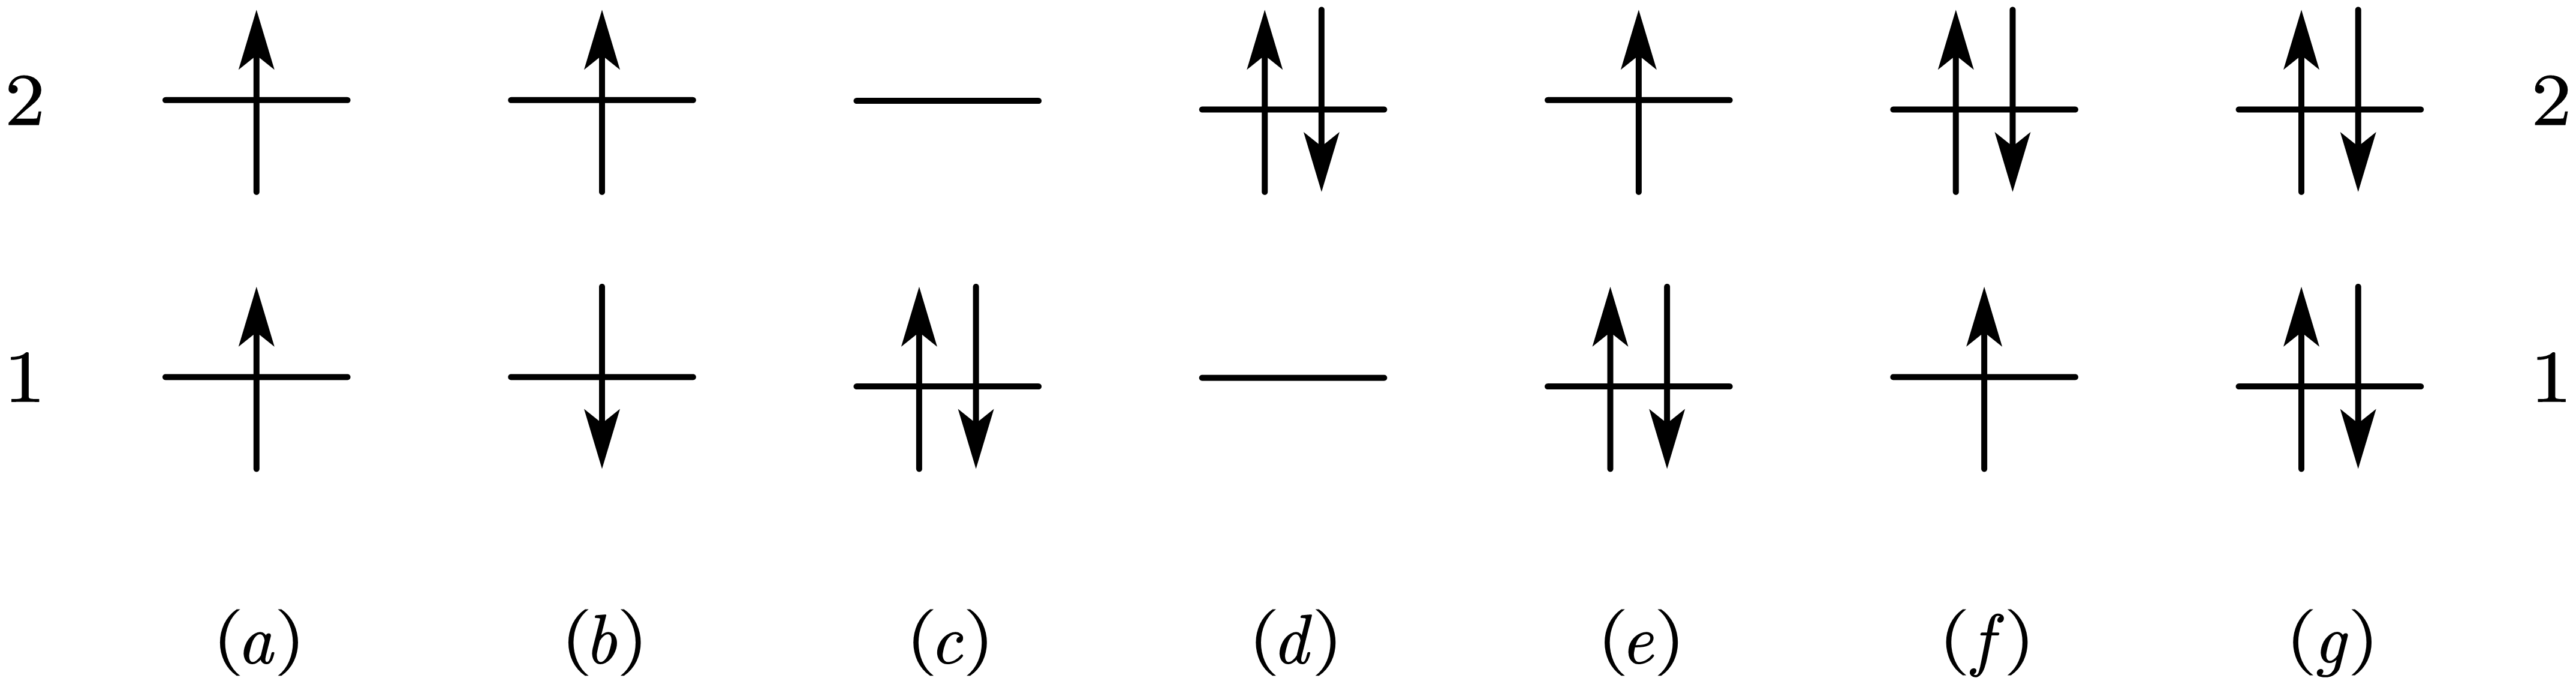
\includegraphics[scale=1.0]{./pictures/2.23/exercise.png}
	\end{center}
	
	\begin{enumerate}
	
	\item[a.] $h_{11} + h_{22} +  J_{12} - K_{12}$.
	
	\item[b.] $h_{11} + h_{22} +  J_{12}$.
	
	\item[c.] $2h_{11} +  J_{11}$.
	
	\item[d.] $2h_{22} +  J_{22}$.
	
	\item[e.] $2h_{11} + h_{22} +  J_{11} + 2J_{12} - K_{12}$.
	
	\item[f.] $2h_{22} + h_{11} +  J_{22} + 2J_{12} - K_{12}$.
	
	\item[g.] $2h_{11} + 2h_{22} +  J_{11} +  J_{22} + 4J_{12} - 2K_{12}$.
	
	\end{enumerate}		
	
	\end{exercise}
	
	\begin{solution}
	
	\begin{itemize}
	
	\item[a.] There are 2 electrons in spatial orbital $1$ and $2$, contributing the terms $h_{11}$ and $h_{22}$. There is only 1 unique pair of electrons in spatial orbitals 1 and 2, contributing the term $J_{12}$. There is only 1 unique pair of electrons with parallel spins in spatial orbitals 1 and 2, contributing the term $-K_{12}$. Thus,
	\[
		E_a = h_{11} + h_{22} +  J_{12} - K_{12}.
	\]
	
	\item[b.] There are 2 electrons in spatial orbital $1$ and $2$, contributing the terms $h_{11}$ and $h_{22}$. There is only 1 unique pair of electrons in spatial orbitals 1 and 2, contributing the term $J_{12}$. However, there is no unique pair of electrons with parallel spins. Thus,
	\[
		E_b = h_{11} + h_{22} +  J_{12} .
	\]
	
	\item[c.] There are 2 electrons both in spatial orbital $1$, contributing the terms $2h_{11}$. There is only 1 unique pair of electrons in spatial orbitals 1, contributing the term $J_{11}$. However, there is no unique pair of electrons with parallel spins. Thus,
	\[
		E_c = 2h_{11} +  J_{11} .
	\]

	\item[d.] There are 2 electrons both in spatial orbital $2$, contributing the terms $2h_{22}$. There is only 1 unique pair of electrons in spatial orbitals 1, contributing the term $J_{22}$. However, there is no unique pair of electrons with parallel spins. Thus,
	\[
		E_d = 2h_{22} +  J_{22} .
	\]
	
	\item[e.] There are 3 electrons in spatial orbital $1$, $1$ and $2$, contributing the terms $h_{11}$, $h_{11}$  and $h_{22}$. There are 3 unique pairs of electrons in spatial orbitals 1 and 1, 1 and 2, 1 and 2, contributing the term $J_{11}$, $J_{12}$ and $J_{12}$. There is only 1 unique pair of electrons with parallel spins in spatial orbitals 1 and 2, contributing the term $-K_{12}$. Thus,
	\[
		E_e = h_{11} + h_{11} + h_{22} + J_{11} + J_{12} + J_{12} - K_{12} = 2h_{11} + h_{22} +  J_{11} + 2J_{12} - K_{12}.
	\]
	
	\item[f.] There are 3 electrons in spatial orbital $1$, $2$ and $2$, contributing the terms $h_{11}$, $h_{22}$  and $h_{22}$. There are 3 unique pairs of electrons in spatial orbitals 1 and 2, 1 and 2, 2 and 2, contributing the term $J_{12}$, $J_{12}$ and $J_{22}$. There is only 1 unique pair of electrons with parallel spins in spatial orbitals 1 and 2, contributing the term $-K_{12}$. Thus,
	\[
		E_f = h_{11} + h_{22} + h_{22} + J_{12} + J_{12} + J_{22} - K_{12} = 2h_{22} + h_{11} +  J_{22} + 2J_{12} - K_{12} .
	\]
	
	\item[g.] There are 4 electrons in spatial orbital $1$, $1$, $2$ and $2$, contributing the terms $h_{11}$, $h_{11}$, $h_{22}$  and $h_{22}$. There are 6 unique pairs of electrons in spatial orbitals 1 and 1, 1 and 2, 1 and 2, 1 and 2, 1 and 2, 2 and 2, contributing the term $J_{11}$, $J_{12}$, $J_{12}$, $J_{12}$, $J_{12}$, and $J_{22}$. There are only 2 unique pair of electrons with parallel spins in spatial orbitals 1 and 2, 1 and 2, contributing the term $-K_{12}$ and $-K_{12}$. Thus,
	\begin{align*}
		E_g &= h_{11} + h_{11} + h_{22} + h_{22} + J_{11} + J_{12} + J_{12} + J_{12} + J_{12} + J_{22} - K_{12} - K_{12} \\
		&= 2h_{11} + 2h_{22} +  J_{11} +  J_{22} + 4J_{12} - 2K_{12} .
	\end{align*}
	
	\end{itemize}		
	
	\end{solution}
	
	\section{Second Quantization}
	
	\subsection{Creation and Annihilation Operators and Their Anticommutation Relations}
	
	% 2.24
	\begin{exercise}
	Show, using the properties of determinants, that
	\[
		( a^\dagger_1 a^\dagger_2 + a^\dagger_2 a^\dagger_1 ) | K \rangle = 0 
	\]
	for every $| K \rangle$ in the set $\{ |\chi_1\chi_2\rangle , |\chi_1\chi_3\rangle , |\chi_1\chi_4\rangle , |\chi_2\chi_3\rangle , |\chi_2\chi_4\rangle , |\chi_3\chi_4\rangle \}$.
	\end{exercise}
	
	\begin{solution}
	
	Using (2.194), the conclusion can be obtained at once.	
	
	\end{solution}
	
	% 2.25
	\begin{exercise}
	Show, using the properties of determinants, that
	\begin{align*}
		( a_1 a^\dagger_2 + a^\dagger_2 a_1 ) | K \rangle &= 0 , \\
		( a_1 a^\dagger_1 + a^\dagger_1 a_1 ) | K \rangle &= | K \rangle
	\end{align*}
	for every $| K \rangle$ in the set $\{ |\chi_1\chi_2\rangle , |\chi_1\chi_3\rangle , |\chi_1\chi_4\rangle , |\chi_2\chi_3\rangle , |\chi_2\chi_4\rangle , |\chi_3\chi_4\rangle \}$.
	\end{exercise}
	
	\begin{solution}
	
	Using (2.217), the conclusion can be obtained at once.
	
	\end{solution}
	
	% 2.26
	\begin{exercise}
	Show using second quantization that $\langle \chi_i | \chi_j \rangle = \delta_{ij}$.
	\end{exercise}
	
	\begin{solution}
	
	The proof is direct.
	\[
		\langle \chi_i | \chi_j \rangle = \langle | a_i a^\dagger_j | \rangle = \langle | \delta_{ij} - a^\dagger_j a_i | \rangle = \delta_{ij} \langle | \rangle - \langle | a^\dagger_j a_i | \rangle = \delta_{ij} .
	\]	
	
	\end{solution}
	
	% 2.27
	\begin{exercise}
	Given a state 
	\[
		| K \rangle = | \chi_1 \chi_2 \cdots \chi_N \rangle = a^\dagger_1 a^\dagger_2 \cdots a^\dagger_N | \rangle,
	\]
	show that $\langle K | a^\dagger_i a_j | K \rangle = 1$ if $i=j$ and $i \in \{ 1 , 2 , \cdots, N \}$, but is zero otherwise.
	\end{exercise}
	
	\begin{solution}
	
	The proof is direct, too.	
	\[
		\langle K | a^\dagger_i a_j | K \rangle = \langle K | \delta_{ij} - a_j a^\dagger_i | K \rangle = \delta_{ij} \langle K | K \rangle - \langle K | a_j a^\dagger_i | K \rangle = \delta_{ij} - \langle K | a_j a^\dagger_i | K \rangle.
	\]	
	It is evident that $\langle K | a^\dagger_i a_j | K \rangle$ will be one if and only if $i=j$ and $i \in \{ 1, 2, \ldots, N \}$. Otherwise, it will be zero.
	
	\end{solution}
	
	% 2.28
	\begin{exercise}
	Let $|\Psi_0\rangle = | \chi_1 \cdots \chi_a \chi_b \cdots \chi_N \rangle$ be the Hartree-Fock ground state wave function. Show that
	\begin{enumerate}
	
	\item[a.] $a_r | \Psi_0 \rangle = 0 = \langle \Psi_0 | a^\dagger_r$.
	
	\item[b.] $a^\dagger_a | \Psi_0 \rangle = 0 = \langle \Psi_0 | a_a$.
	
	\item[c.] $| \Psi^r_a \rangle = a^\dagger_r a_a | \Psi_0 \rangle $.
	
	\item[d.] $\langle \Psi^r_a | = \langle \Psi_0 | a^\dagger_a a_r$.
	
	\item[e.] $| \Psi^{rs}_{ab} \rangle = a^\dagger_s a_b a^\dagger_r a_a | \Psi_0 \rangle = a^\dagger_r a^\dagger_s a_b  a_a | \Psi_0 \rangle $.
	
	\item[f.] $\langle \Psi^{rs}_{ab} | = \langle \Psi_0 | a^\dagger_a a_r a^\dagger_b a_s = \langle \Psi_0 | a^\dagger_a a^\dagger_b a_s a_r$.
	
	\end{enumerate}
	\end{exercise}
	
	\begin{solution}
	
	Assume that $a$, $b$ are labels of occupied spin orbitals while $r$, $s$ are labels of unoccupied spin orbitals.
	
	\begin{itemize}

	\item[a.] It is evident because there exists no electron occupying spin orbital $r$.
	
	\item[b.] It is also evident because there is an electron occupying spin orbital $a$.
	
	\item[c.] The verification is direct.
	\begin{align*}
		 | \Psi^r_a \rangle &= | \chi_1 \cdots \chi_r \chi_b \cdots \chi_N \rangle = - | \chi_r \cdots \chi_1 \chi_b \cdots \chi_N \rangle = - a^\dagger_r | \cdots \chi_1 \chi_b \cdots \chi_N \rangle \\
		 &=  - a^\dagger_r a_a | \chi_a \cdots \chi_1 \chi_b \cdots \chi_N \rangle = a^\dagger_r a_a | \chi_1 \cdots \chi_a \chi_b \cdots \chi_N \rangle = a^\dagger_r a_a | \Psi_0 \rangle .
	\end{align*}
	
	\item[d.] The verification is direct, too.
	\begin{align*}
		\langle \Psi^r_a | &= \langle \chi_1 \cdots \chi_r \chi_b \cdots \chi_N | = - \langle \chi_1 \cdots \chi_N \chi_b \cdots \chi_r | = - \langle \chi_1 \cdots \chi_N \chi_b \cdots | a_r \\
		&= -  \langle \chi_1 \cdots \chi_N \chi_b \cdots \chi_a | a^\dagger_a a_r = \langle \chi_1 \cdots \chi_a \chi_b \cdots \chi_N | a^\dagger_a a_r = \langle \Psi_0 | a^\dagger_a a_r . 
	\end{align*}
	
	
	\item[e.] The verification is direct, too.
	\begin{align*}
		| \Psi^{rs}_{ab} \rangle &= | \chi_1 \chi_2 \cdots \chi_r \chi_s \cdots \chi_N \rangle = (-1)^2 | \chi_r \chi_s \cdots \chi_1 \chi_2 \cdots \chi_N \rangle = a^\dagger_r | \chi_s \cdots \chi_1 \chi_2 \cdots \chi_N \rangle \\
		&= a^\dagger_r a^\dagger_s | \cdots \chi_1 \chi_2 \cdots \chi_N \rangle = a^\dagger_r a^\dagger_s a_b | \chi_b \cdots \chi_1 \chi_2 \cdots \chi_N \rangle = - a^\dagger_r a^\dagger_s a_b | \chi_2 \cdots \chi_1 \chi_b \cdots \chi_N \rangle \\
		&= - a^\dagger_r a^\dagger_s a_b a_a | \chi_a \chi_2 \cdots \chi_1 \chi_b \cdots \chi_N \rangle = a^\dagger_r a^\dagger_s a_b a_a | \chi_1 \chi_2 \cdots \chi_a \chi_b \cdots \chi_N \rangle = a^\dagger_r a^\dagger_s a_b a_a | \Psi_0 \rangle .
	\end{align*}		
	Note that with $\delta_{ar} = \delta_{br} = \delta_{as} = \delta_{bs} = 0$, 
	\[
		a^\dagger_r a^\dagger_s a_b = - a^\dagger_s a^\dagger_r a_b = - a^\dagger_s ( \delta_{br} - a_b a^\dagger_r ) = a^\dagger_s a_b a^\dagger_r .
	\]
	We obtain that
	\[
		| \Psi^{rs}_{ab} \rangle = a^\dagger_r a^\dagger_s a_b a_a | \Psi_0 \rangle = a^\dagger_s a_b a^\dagger_r a_a | \Psi_0 \rangle .
	\]
	
	\item[f.] The verification is direct, too.
	\begin{align*}
		\langle \Psi^{rs}_{ab} | &= \langle \chi_1 \cdots \chi_r \chi_s \cdots \chi_{N-1} \chi_N | = (-1)^2 \langle \chi_1 \cdots \chi_N \chi_{N-1} \cdots \chi_s \chi_r | = \langle \chi_1 \cdots \chi_N \chi_{N-1} \cdots \chi_s | a_r \\
		&= \langle \chi_1 \cdots \chi_N \chi_{N-1} \cdots | a_s a_r = \langle \chi_1 \cdots \chi_N \chi_{N-1} \cdots \chi_b | a^\dagger_b a_s a_r = - \langle \chi_1 \cdots \chi_N \chi_b \cdots \chi_{N-1} | a^\dagger_b a_s a_r \\
		&= - \langle \chi_1 \cdots \chi_N \chi_b \cdots \chi_{N-1} \chi_a | a^\dagger_a a^\dagger_b a_s a_r = \langle \chi_1 \cdots \chi_a \chi_b \cdots \chi_{N-1} \chi_N | a^\dagger_a a^\dagger_b a_s a_r = \langle \Psi_0 | a^\dagger_a a^\dagger_b a_s a_r .
	\end{align*}
	
	In the same way, we can find that
	\[
		a^\dagger_b a_s a_r = - a^\dagger_b a_r a_s = - ( \delta_{br} - a_r a^\dagger_b ) a_s = a_r a^\dagger_b a_s .
	\]	
	Thus, 
	\[
		\langle \Psi^{rs}_{ab} | = \langle \Psi_0 | a^\dagger_a a^\dagger_b a_s a_r = \langle \Psi_0 | a^\dagger_a a_r a^\dagger_b a_s .
	\]
	
	\end{itemize}
	
	\end{solution}
	
	\subsection{Second-Quantized Operators and Their Matrix Elements}
	
	% 2.29
	\begin{exercise}
	Let $| \Psi_0 \rangle = | \chi_1 \chi_2 \rangle = a^\dagger_1 a^\dagger_2 | \rangle$ be the Hartree-Fock wave function for minimal basis $\ce{H2}$. Show using second quantization that
	\[
		\langle \Psi_0 | \mathscr{O}_1 | \Psi_0 \rangle = \sum_{ij} \langle i | h | j \rangle \langle | a_2 a_1 a^\dagger_i a_j a^\dagger_1 a^\dagger_2 | \rangle = \langle 1 | h | 1 \rangle + \langle 2 | h | 2 \rangle.
	\]
	\end{exercise}
	
	\begin{solution}
	
	Using (2.231) and the conclusion of Exercise 2.28, we find that
	\begin{align*}
		&\hspace{1.4em}\langle \Psi_0 | \mathscr{O}_1 | \Psi_0 \rangle = \langle \chi_1 \chi_2 | \sum_{ij} \langle i | h | j \rangle a^\dagger_i a_j | \chi_1 \chi_2 \rangle = \sum_{ij} \langle i | h | j \rangle \langle | a_2 a_1 a^\dagger_i a_j a^\dagger_1 a^\dagger_2 | \rangle \\
		&= \sum_{ij} \langle i | h | j \rangle \langle | a_2 ( \delta_{1i} - a^\dagger_i a_1 ) ( \delta_{j1} - a^\dagger_1 a_j ) a^\dagger_2 | \rangle \\
		&= \sum_{ij} \langle i | h | j \rangle \left[ \delta_{1i} \delta_{1j} \langle | a_2 a^\dagger_2 | \rangle - \delta_{1i} \langle | a_2 a^\dagger_1 a_j a^\dagger_2 | \rangle - \delta_{j1} \langle | a_2 a^\dagger_i a_1 a^\dagger_2 | \rangle + \langle | a_2 a^\dagger_i a_1 a^\dagger_1 a_j a^\dagger_2 | \rangle \right] \\
		&= \langle 1 | h | 1 \rangle \langle | a_2 a^\dagger_2 | \rangle - \sum_j \langle 1 | h | j \rangle \langle | a_2 a^\dagger_1 a_j a^\dagger_2 | \rangle - \sum_i \langle i | h | 1 \rangle \langle | a_2 a^\dagger_i a_1 a^\dagger_2 | \rangle + \sum_{ij} \langle i | h | j \rangle \langle | a_2 a^\dagger_i a_1 a^\dagger_1 a_j a^\dagger_2 | \rangle \\
		&= \langle 1 | h | 1 \rangle \left( \langle | \delta_{22} - a^\dagger_2 a_2 | \rangle \right) - \sum_j \langle 1 | h | j \rangle \langle | ( \delta_{12} - a^\dagger_1 a_2 )  a_j a^\dagger_2 | \rangle - \sum_i \langle i | h | 1 \rangle \langle | a_2 a^\dagger_i ( \delta_{12} - a^\dagger_2 a_1 ) | \rangle \\
		&\hspace{4em} + \sum_{ij} \langle i | h | j \rangle \langle | ( \delta_{2i} - a^\dagger_i a_2 ) a_1 a^\dagger_1 ( \delta_{2j} - a^\dagger_2 a_j ) | \rangle \\
		&= \langle 1 | h | 1 \rangle \left( 1 - 0 \right) + \sum_j \langle 1 | h | j \rangle \langle | a^\dagger_1 a_2 a_j a^\dagger_2 | \rangle + \sum_i \langle i | h | 1 \rangle \langle | a_2 a^\dagger_i a^\dagger_2 a_1 | \rangle \\
		&\hspace{4em} + \sum_{ij} \langle i | h | j \rangle \left[ \delta_{2i} \delta_{2j} \langle | a_1 a^\dagger_1 | \rangle - \delta_{2i} \langle | a_1 a^\dagger_1 a^\dagger_2 a_j | \rangle - \delta_{2j} \langle | a^\dagger_i a_2 a_1 a^\dagger_1 | \rangle + \langle | a^\dagger_i a_2 a_1 a^\dagger_1 a^\dagger_2 a_j | \rangle \right] \\
		&= \langle 1 | h | 1 \rangle + 0 + 0 + \langle 2 | h | 2 \rangle ( \delta_{11} - \langle | a_1 a^\dagger_1 | \rangle ) - 0 - 0 + 0 = \langle 1 | h | 1 \rangle + \langle 2 | h | 2 \rangle ( 1 - 0 ) = \langle 1 | h | 1 \rangle + \langle 2 | h | 2 \rangle.
	\end{align*}		
	
	\end{solution}
	
	% 2.30
	\begin{exercise}
	Show that
	\[
		\langle \Psi^r_a | \mathscr{O}_1 | \Psi_0 \rangle = \sum_{ij} \langle i | h | j \rangle \langle \Psi_0 | a^\dagger_a a_r a^\dagger_i a_j | \Psi_0 \rangle = \langle r | h | a \rangle
	\]
	by moving $a^\dagger_a$ and $a_r$ to the right.
	\end{exercise}
	
	\begin{solution}
	
	Using (2.231) and the conclusion of Exercise 2.28, we find that
	\begin{align*}
		&\hspace{1.4em}\langle \Psi^r_a | \mathscr{O}_1 | \Psi_0 \rangle = \langle \Psi_0 | a^\dagger_a a_r \sum_{ij} \langle i | h | j \rangle a^\dagger_i a_j | \Psi_0 \rangle = \sum_{ij} \langle i | h | j \rangle \langle \Psi_0 | a^\dagger_a a_r a^\dagger_i a_j | \Psi_0 \rangle \\
		&= \sum_{ij} \langle i | h | j \rangle \langle \Psi_0 | a^\dagger_a ( \delta_{ri} - a^\dagger_i a_r ) a_j | \Psi_0 \rangle = \sum_j \langle r | h | j \rangle \langle \Psi_0 | a^\dagger_a a_j | \Psi_0 \rangle - \sum_{ij} \langle i | h | j \rangle \langle \Psi_0 | a^\dagger_a a^\dagger_i a_r a_j | \Psi_0 \rangle \\
		&= \sum_j \langle r | h | j \rangle \langle \Psi_0 | ( \delta_{aj} - a_j a^\dagger_a ) | \Psi_0 \rangle + \sum_{ij} \langle i | h | j \rangle \langle \Psi_0 | a^\dagger_a a^\dagger_i a_j a_r | \Psi_0 \rangle \\
		&= \sum_j \langle r | h | j \rangle \delta_{aj} - \sum_j \langle r | h | j \rangle \langle \Psi_0 | a_j a^\dagger_a | \Psi_0 \rangle + 0 = \langle r | h | a \rangle + 0 = \langle r | h | a \rangle .
	\end{align*}
	
	\end{solution}
	
	% 2.31
	\begin{exercise}
	Show that
	\[
		\langle \Psi^r_a | \mathscr{O}_2 | \Psi_0 \rangle = \sum_b^N \langle rb || ab \rangle .
	\]
	{\it Hint}: first show that
	\begin{align*}
		\langle \Psi_0 | a^\dagger_a a_r a^\dagger_i a^\dagger_j a_l a_k | \Psi_0 \rangle &= \delta_{rj} \delta_{al} \langle \Psi_0 | a^\dagger_i a_k | \Psi_0 \rangle - \delta_{rj} \delta_{ak} \langle \Psi_0 | a^\dagger_i a_l | \Psi_0 \rangle \\
		&\hspace{4em} + \delta_{ri} \delta_{ak} \langle \Psi_0 | a^\dagger_j a_l | \Psi_0 \rangle - \delta_{ri} \delta_{al} \langle \Psi_0 | a^\dagger_j a_k | \Psi_0 \rangle
	\end{align*}
	then refer to Exercise 2.27.
	\end{exercise}
	
	\begin{solution}
	
	Similar to Exercise 2.30, we find that
	\begin{align*}
		&\hspace{1.4em}\langle \Psi_0 | a^\dagger_a a_r a^\dagger_i a^\dagger_j a_l a_k | \Psi_0 \rangle \\
		&= \langle \Psi_0 | a^\dagger_a ( \delta_{ri} - a^\dagger_i a_r ) a^\dagger_j a_l a_k | \Psi_0 \rangle = \delta_{ri} \langle \Psi_0 | a^\dagger_a a^\dagger_j a_l a_k | \Psi_0 \rangle - \langle \Psi_0 | a^\dagger_a a^\dagger_i a_r a^\dagger_j a_l a_k | \Psi_0 \rangle \\
		&= - \delta_{ri} \langle \Psi_0 | a^\dagger_j a^\dagger_a a_l a_k | \Psi_0 \rangle - \langle \Psi_0 | a^\dagger_a a^\dagger_i ( \delta_{rj} - a^\dagger_j a_r ) a_l a_k | \Psi_0 \rangle \\
		&= - \delta_{ri} \langle \Psi_0 | a^\dagger_j ( \delta_{al} - a_l a^\dagger_a ) a_k | \Psi_0 \rangle - \delta_{rj} \langle \Psi_0 | a^\dagger_a a^\dagger_i a_l a_k | \Psi_0 \rangle + \langle \Psi_0 | a^\dagger_a a^\dagger_i a^\dagger_j a_r a_l a_k | \Psi_0 \rangle  \\
		&= - \delta_{ri} \delta_{al} \langle \Psi_0 | a^\dagger_j a_k | \Psi_0 \rangle + \delta_{ri} \langle \Psi_0 | a^\dagger_j a_l a^\dagger_a a_k | \Psi_0 \rangle + \delta_{rj} \langle \Psi_0 | a^\dagger_i a^\dagger_a a_l a_k | \Psi_0 \rangle - \langle \Psi_0 | a^\dagger_a a^\dagger_i a^\dagger_j a_l a_r a_k | \Psi_0 \rangle \\
		&= - \delta_{ri} \delta_{al} \langle \Psi_0 | a^\dagger_j a_k | \Psi_0 \rangle + \delta_{ri} \langle \Psi_0 | a^\dagger_j a_l ( \delta_{ak} - a_k a^\dagger_a ) | \Psi_0 \rangle \\
		&\hspace{4em} + \delta_{rj} \langle \Psi_0 | a^\dagger_i ( \delta_{al} - a_l a^\dagger_a ) a_k | \Psi_0 \rangle + \langle \Psi_0 | a^\dagger_a a^\dagger_i a^\dagger_j a_l a_k a_r | \Psi_0 \rangle \\
		&= - \delta_{ri} \delta_{al} \langle \Psi_0 | a^\dagger_j a_k | \Psi_0 \rangle + \delta_{ri} \delta_{ak} \langle \Psi_0 | a^\dagger_j a_l | \Psi_0 \rangle - \delta_{ri} \langle \Psi_0 | a^\dagger_j a_l a_k a^\dagger_a | \Psi_0 \rangle \\
		&\hspace{4em} + \delta_{rj} \delta_{al} \langle \Psi_0 | a^\dagger_i a_k | \Psi_0 \rangle - \delta_{rj} \langle \Psi_0 | a^\dagger_i a_l a^\dagger_a a_k | \Psi_0 \rangle + 0 \\
		&= - \delta_{ri} \delta_{al} \langle \Psi_0 | a^\dagger_j a_k | \Psi_0 \rangle + \delta_{ri} \delta_{ak} \langle \Psi_0 | a^\dagger_j a_l | \Psi_0 \rangle - 0 + \delta_{rj} \delta_{al} \langle \Psi_0 | a^\dagger_i a_k | \Psi_0 \rangle - \delta_{rj} \langle \Psi_0 | a^\dagger_i a_l ( \delta_{ak} - a_k a^\dagger_a ) | \Psi_0 \rangle \\
		&= - \delta_{ri} \delta_{al} \langle \Psi_0 | a^\dagger_j a_k | \Psi_0 \rangle + \delta_{ri} \delta_{ak} \langle \Psi_0 | a^\dagger_j a_l | \Psi_0 \rangle \\
		&\hspace{4em} + \delta_{rj} \delta_{al} \langle \Psi_0 | a^\dagger_i a_k | \Psi_0 \rangle - \delta_{rj} \delta_{ak} \langle \Psi_0 | a^\dagger_i a_l | \Psi_0 \rangle + \delta_{rj} \langle \Psi_0 | a^\dagger_i a_l a_k a^\dagger_a | \Psi_0 \rangle  \\
		&= \delta_{rj} \delta_{al} \langle \Psi_0 | a^\dagger_i a_k | \Psi_0 \rangle - \delta_{rj} \delta_{ak} \langle \Psi_0 | a^\dagger_i a_l | \Psi_0 \rangle + \delta_{ri} \delta_{ak} \langle \Psi_0 | a^\dagger_j a_l | \Psi_0 \rangle - \delta_{ri} \delta_{al} \langle \Psi_0 | a^\dagger_j a_k | \Psi_0 \rangle .
	\end{align*}
	
	Note that $\langle \Psi_0 | a^\dagger_i a_j | \Psi_0 \rangle$ equals 1 if and only if $i$ and $j$ is should be labels of occupied spin orbitals like $a$ and $b$. Hence, we find that
	\begin{align*}
		&\hspace{1.4em}\langle \Psi^r_a | \mathscr{O}_2 | \Psi_0 \rangle = \langle \Psi_0 | a^\dagger_a a_r \frac{1}{2}\sum_{ijkl} \langle ij | kl \rangle a^\dagger_i a^\dagger_j a_l a_k | \Psi_0 \rangle = \frac{1}{2} \sum_{ijkl} \langle ij | kl \rangle \langle \Psi_0 | a^\dagger_a a_r a^\dagger_i a^\dagger_j a_l a_k  | \Psi_0 \rangle \\
		&= \frac{1}{2} \sum_{ijkl} \langle ij | kl \rangle ( \delta_{rj} \delta_{al} \langle \Psi_0 | a^\dagger_i a_k | \Psi_0 \rangle - \delta_{rj} \delta_{ak} \langle \Psi_0 | a^\dagger_i a_l | \Psi_0 \rangle + \delta_{ri} \delta_{ak} \langle \Psi_0 | a^\dagger_j a_l | \Psi_0 \rangle - \delta_{ri} \delta_{al} \langle \Psi_0 | a^\dagger_j a_k | \Psi_0 \rangle ) \\
		&= \frac{1}{2} \sum_{ik} \langle ir | ka \rangle \langle \Psi_0 | a^\dagger_i a_k | \Psi_0 \rangle - \frac{1}{2} \sum_{il} \langle ir | al \rangle \langle \Psi_0 | a^\dagger_i a_l | \Psi_0 \rangle \\
		&\hspace{4em} + \frac{1}{2} \sum_{jl} \langle rj | al \rangle \langle \Psi_0 | a^\dagger_j a_l | \Psi_0 \rangle - \frac{1}{2} \sum_{jk} \langle rj | ka \rangle \langle \Psi_0 | a^\dagger_j a_k | \Psi_0 \rangle \\
		&= \frac{1}{2} \sum_{ij} \langle ir | ja \rangle \langle \Psi_0 | a^\dagger_i a_j | \Psi_0 \rangle - \frac{1}{2} \sum_{ij} \langle ir | aj \rangle \langle \Psi_0 | a^\dagger_i a_j | \Psi_0 \rangle \\
		&\hspace{4em} + \frac{1}{2} \sum_{ij} \langle ri | aj \rangle \langle \Psi_0 | a^\dagger_i a_j | \Psi_0 \rangle - \frac{1}{2} \sum_{ij} \langle ri | ja \rangle \langle \Psi_0 | a^\dagger_i a_j | \Psi_0 \rangle \\
		&= \sum_{ij} \langle ir | ja \rangle \langle \Psi_0 | a^\dagger_i a_j | \Psi_0 \rangle - \langle ir | aj \rangle \langle \Psi_0 | a^\dagger_i a_j | \Psi_0 \rangle = \sum_{ij} \langle ir || ja \rangle \langle \Psi_0 | a^\dagger_i a_j | \Psi_0 \rangle \\
		&= \sum_{ij} \langle ri || aj \rangle \langle \Psi_0 | a^\dagger_i a_j | \Psi_0 \rangle = \sum_b^N \langle rb || ab \rangle .
	\end{align*}
	
	\end{solution}
	
	\section{Spin-Adapted Configurations}
	
	\subsection{Spin Operators}
	
	% 2.32
	\begin{exercise}
	a) Derive (2.247) from (2.245); b) Derive (2.248).
	\end{exercise}
	
	\begin{solution}
	
	\begin{itemize}
	
	\item[a)] Using (2.246a) and (2.245c,d), we find that
	\begin{align*}
		s_+ | \alpha \rangle &= ( s_x + i s_y ) | \alpha \rangle = s_x | \alpha \rangle + i s_y | \alpha \rangle = \frac{1}{2} | \beta \rangle + i \times \frac{ i }{ 2 } | \beta \rangle = \left( \frac{1}{2} + i \times \frac{ i }{ 2 } \right) | \beta \rangle = 0 , \\
		s_+ | \beta \rangle &= ( s_x + i s_y ) | \beta \rangle = s_x | \beta \rangle + i s_y | \beta \rangle = \frac{1}{2} | \alpha \rangle + i \times \frac{ -i }{ 2 } | \alpha \rangle = \left( \frac{1}{2} + i \times \frac{ -i }{ 2 } \right) | \alpha \rangle = | \alpha \rangle , \\
		s_- | \alpha \rangle &= ( s_x - i s_y ) | \alpha \rangle = s_x | \alpha \rangle - i s_y | \alpha \rangle = \frac{1}{2} | \beta \rangle - i \times \frac{ i }{ 2 } | \beta \rangle = \left( \frac{1}{2} - i \times \frac{ i }{ 2 } \right) | \beta \rangle = | \beta \rangle , \\
		s_- | \beta \rangle &= ( s_x - i s_y ) | \beta \rangle = s_x | \beta \rangle - i s_y | \beta \rangle = \frac{1}{2} | \alpha \rangle - i \times \frac{ -i }{ 2 } | \alpha \rangle = \left( \frac{1}{2} - i \times \frac{ -i }{ 2 } \right) | \alpha \rangle = 0 .
	\end{align*}
	
	\item[b)] From (2.246a,b) and the conclusion of Exercise 1.4(f), we know that
	\[
		\begin{pmatrix}
			s_+ \\ s_- 
		\end{pmatrix} = \begin{pmatrix}
			1 & i \\
			1 & -i
		\end{pmatrix} \begin{pmatrix}
			s_x \\ s_y
		\end{pmatrix} \Leftrightarrow \begin{pmatrix}
			s_x \\ s_y
		\end{pmatrix} = \begin{pmatrix}
			1 & i \\
			1 & -i
		\end{pmatrix}^{-1} \begin{pmatrix} 
			s_+ \\ s_- 
		\end{pmatrix} = \frac{1}{-2i} \begin{pmatrix}
			-i & -i \\
			-1 & 1
		\end{pmatrix} \begin{pmatrix} 
			s_+ \\ s_- 
		\end{pmatrix} .
	\]
	In other words, we know that
	\[
		s_x = \frac{ -i s_+ -i s_- }{-2i} = \frac{ s_+ + s_- }{2} , \quad s_y = \frac{ - s_+ + s_- }{-2i} = \frac{ s_+ - s_- }{2i} .
	\]
	Besides, with (2.242), it is evident that
	\[
		[ s_+ , s_- ] = [ s_x + i s_y , s_x - i s_y ] = [ s_x , s_x ] - i [ s_x , s_y ] + i [ s_y , s_x ] + [ s_y , s_y ] = -2i [ s_x , s_y ] = -2i ( is_z ) = 2 s_z .
	\]
	
	From (2.241), we find that
	\begin{align*}
		s^2 &= s^2_x + s^2_y + s^2_z = \left( \frac{ s_+ + s_- }{2} \right)^2 + \left( \frac{ s_+ - s_- }{2i} \right)^2 + s^2_z \\
		&= \frac{1}{4} \left( s^2_+ + s_+ s_- + s_- s_+ + s^2_- \right) - \frac{1}{4} \left( s^2_+ - s_+ s_- - s_- s_+ + s^2_- \right) + s^2_z \\
		&= \frac{1}{2} \left( s_+ s_- + s_- s_+ \right) + s^2_z = s_+ s_- + \frac{1}{2} \left( s_- s_+ -  s_+ s_- \right) + s^2_z = s_- s_+ + \frac{1}{2} \left( s_+ s_- -  s_- s_+ \right) + s^2_z \\
		&= s_+ s_- + \frac{1}{2} [ s_- , s_+ ] + s^2_z = s_+ s_- - \frac{1}{2} [ s_+ , s_- ] + s^2_z = s_+ s_- - \frac{1}{2} (2s_z) + s^2_z =  s_+ s_- - s_z + s^2_z \\
		&= s_- s_+ + \frac{1}{2} [ s_+ , s_- ] + s^2_z = s_- s_+ + \frac{1}{2}(2s_z) + s^2_z =  s_- s_+ + s_z + s^2_z .
	\end{align*}

	\end{itemize}		
	
	\end{solution}
	
	% 2.33
	\begin{exercise}
	Find the $2 \times 2$ matrix representations of $s^2$, $s_z$, $s_+$, and $s_-$ in the basis $|\alpha\rangle$, $|\beta\rangle$. Verify the identities analogous to (2.248a,b) for these matrix representations.
	\end{exercise}
	
	\begin{solution}
	
	From (2.245a,b,c,d), at once we get that
	\begin{align*}
		s^2 ( | \alpha \rangle , | \beta \rangle ) &= ( | \alpha \rangle , | \beta \rangle )	\begin{pmatrix}
		\frac{3}{4} & 0 \\ 0 & \frac{3}{4}
		\end{pmatrix} , \\
		s_z ( | \alpha \rangle , | \beta \rangle ) &= ( | \alpha \rangle , | \beta \rangle )	\begin{pmatrix}
		\frac{1}{2} & 0 \\ 0 & -\frac{1}{2}
		\end{pmatrix} , \\
		s_x ( | \alpha \rangle , | \beta \rangle ) &= ( | \alpha \rangle , | \beta \rangle )	\begin{pmatrix}
		0 & \frac{1}{2} \\ \frac{1}{2} & 0
		\end{pmatrix} , \\
		s_y ( | \alpha \rangle , | \beta \rangle ) &= ( | \alpha \rangle , | \beta \rangle )	\begin{pmatrix}
		0 & -\frac{i}{2} \\ \frac{i}{2} & 0
		\end{pmatrix} .
	\end{align*}
	Thus, we find that
	\begin{align*}
		s_+ ( | \alpha \rangle , | \beta \rangle ) &= ( s_x + i s_y ) ( | \alpha \rangle , | \beta \rangle ) = s_x ( | \alpha \rangle , | \beta \rangle ) + i s_y ( | \alpha \rangle , | \beta \rangle ) \\
		&= ( | \alpha \rangle , | \beta \rangle )	\begin{pmatrix}
		0 & \frac{1}{2} \\ \frac{1}{2} & 0
		\end{pmatrix} + ( | \alpha \rangle , | \beta \rangle )	\left[ i \begin{pmatrix}
		0 & -\frac{i}{2} \\ \frac{i}{2} & 0
		\end{pmatrix} \right] = ( | \alpha \rangle , | \beta \rangle )	\begin{pmatrix}
		0 & 1 \\ 0 & 0
		\end{pmatrix} . \\
		s_- ( | \alpha \rangle , | \beta \rangle ) &= ( s_x - i s_y ) ( | \alpha \rangle , | \beta \rangle ) = s_x ( | \alpha \rangle , | \beta \rangle ) - i s_y ( | \alpha \rangle , | \beta \rangle ) \\
		&= ( | \alpha \rangle , | \beta \rangle )	\begin{pmatrix}
		0 & \frac{1}{2} \\ \frac{1}{2} & 0
		\end{pmatrix} + ( | \alpha \rangle , | \beta \rangle )	\left[ -i \begin{pmatrix}
		0 & -\frac{i}{2} \\ \frac{i}{2} & 0
		\end{pmatrix} \right] = ( | \alpha \rangle , | \beta \rangle )	\begin{pmatrix}
		0 & 0 \\ 1 & 0
		\end{pmatrix} .
	\end{align*}
	Thus, in the basis $|\alpha\rangle$, $|\beta\rangle$, the $2 \times 2$ matrix representations of $s^2$, $s_z$, $s_+$ and $s_-$ are
	\begin{sequation}
		s^2 = \begin{pmatrix}
		\frac{3}{4} & 0 \\ 0 & \frac{3}{4}
		\end{pmatrix} , \quad 
		s_z = \begin{pmatrix}
		\frac{1}{2} & 0 \\ 0 & -\frac{1}{2}
		\end{pmatrix} , \quad 
		s_+ = \begin{pmatrix}
		0 & 1 \\ 0 & 0
		\end{pmatrix} , \quad 
		s_- = \begin{pmatrix}
		0 & 0 \\ 1 & 0
		\end{pmatrix} .
	\end{sequation}
	
	Readers can verify that these matrices represent identities similar to (2.248a,b) by themselves.
	
	\end{solution}
	
	% 2.34
	\begin{exercise}
	Using the commutation relations (2.242), show that $[s^2, s_z] = 0$.
	\end{exercise}
	
	\begin{solution}
	
	Before verification, note that for any operators (matrices) $A$, $B$, $C$,
	\begin{align*}
		[AB,C] &= ABC - CAB = ABC - ACB + ACB - CAB \\
		&= A( BC - CB ) + ( AC - CA )B = A[B,C] + [A,C]B.
	\end{align*}

	From (2.241) and (2.242), we find that
	\begin{align*}
		[s^2, s_z] &= [ s^2_x + s^2_y + s^2_z , s_z ] = [ s^2_x , s_z ] + [ s^2_y , s_z ] + [ s^2_z , s_z ] \\
		&= s_x [ s_x , s_z ] + [ s_x , s_z ] s_x + s_y [ s_y , s_z ] + [ s_y , s_z ] s_y + s_z [ s_z , s_z ] + [ s_z , s_z ] s_z \\
		&= - s_x [ s_z , s_x ] - [ s_z , s_x ] s_x + s_y [ s_y , s_z ] + [ s_y , s_z ] s_y + 0 + 0 \\
		&= - s_x ( i s_y ) - ( i s_y ) s_x + s_y ( i s_x ) + ( i s_x ) s_y = ( -i + i ) s_x s_y + ( -i + i ) s_y s_x = 0.
	\end{align*}

	\end{solution}
	
	% 2.35
	\begin{exercise}
	Consider an operator $\mathscr{A}$ that commutes with the Hamiltonian. Suppose $|\Phi\rangle$ is an eigenfunction of $\mathscr{H}$ with eigenvalue $E$. Show that $\mathscr{A}|\Phi\rangle$ is also an eigenfunction of $\mathscr{H}$ with eigenvalue $E$. Thus if $|\Phi\rangle$ is (energetically) nondegenerate, then $\mathscr{A}|\Phi\rangle$ is at most a constant multiple of $|\Phi\rangle$ (i.e., $\mathscr{A}|\Phi\rangle = a|\Phi\rangle$) and hence $|\Phi\rangle$ is an eigenfunction of $\mathscr{A}$. In case of degeneracies, we can always construct appropriate linear combinations of the degenerate eigenfunctions of $\mathscr{H}$ that are also eigenfunctions of $\mathscr{A}$.
	\end{exercise}
	
	\begin{solution}
	
	The proof of that if an operator $\mathscr{A}$ that commutes with the Hamiltonian and $|\Phi\rangle$ is an eigenfunction of $\mathscr{H}$ with eigenvalue $E$, $\mathscr{A}|\Phi\rangle$ will be also an eigenfunction of $\mathscr{H}$ with eigenvalue $E$, is easy.
	\[
		\mathscr{H} \mathscr{A} |\Phi\rangle = \mathscr{A} \mathscr{H} |\Phi\rangle = \mathscr{A} E |\Phi\rangle = E \mathscr{A} |\Phi\rangle .
	\]
	
	\end{solution}
	
	% 2.36
	\begin{exercise}
	Given two nondegenerate eigenfunctions of a hermitian operator $\mathscr{A}$ that commutes with $\mathscr{H}$, i.e., $\mathscr{A} | \Psi_1 \rangle = a_1 | \Psi_1 \rangle$, $\mathscr{A} | \Psi_2 \rangle = a_2 | \Psi_2 \rangle$, $a_1 \neq a_2$, show that $\langle \Psi_1 | \mathscr{H} | \Psi_2 \rangle = 0$. Thus the matrix element of the Hamiltonian between, say, singlet and triplet spin-adapted configurations is zero.
	\end{exercise}
	
	\begin{solution}
	
	As $\mathscr{A}$ is a hermitian operator, $a_1$ and $a_2$ are real and
	\[
		\langle \Psi_2 | \mathscr{A} = a_2 \langle \Psi_2 |.
	\]
	Hence, 
	\[
		a_1 \langle \Psi_2 | \mathscr{H} | \Psi_1 \rangle = \langle \Psi_2 | \mathscr{H} a_1 | \Psi_1 \rangle = \langle \Psi_2 | \mathscr{H} \mathscr{A} | \Psi_1 \rangle = \langle \Psi_2 | \mathscr{A} \mathscr{H} | \Psi_1 \rangle = a_2 \langle \Psi_2 | \mathscr{H} | \Psi_1 \rangle .
	\]
	In other words,
	\[
		( a_1 - a_2 ) \langle \Psi_2 | \mathscr{H} | \Psi_1 \rangle = 0 .
	\]
	Due to $a_1 \neq a_2$, we find that
	\[
		\langle \Psi_1 | \mathscr{H} | \Psi_2 \rangle = 0 .
	\]

	\end{solution}
	
	% 2.37
	\begin{exercise}
	Prove Eq.(2.254). {\it Hint:} Use expansion (2.115) for a Slater determinant and note that $\mathscr{S}_z$, since it is invariant to any permutation of the electron labels, commutes with $\mathscr{P}_n$.
	\end{exercise}
	
	\begin{solution}
	
	Firstly, note that
	\begin{align*}
		s_z(i) \chi_j( \bfx_i ) = \frac{ \delta_{j\alpha} - \delta_{j\beta} }{2} \chi_j( \bfx_i ) .
	\end{align*}
	
	The derivation is exactly the same as that of Exercise 2.15 if $h(i)$ is replaced by $s_z(i)$. And thus, $\sum_{ i=1 }^N \varepsilon_i$ should be replaced by
	\[
		\sum_{ i=1 }^N \frac{ \delta_{j\alpha} - \delta_{j\beta} }{2} = \frac{ N^\alpha - N^\beta }{2} .
	\]
	
	\end{solution}
	
	\subsection{Restricted Determinants and Spin-Adapted Configurations}
	
	% 2.38
	\begin{exercise}
	Prove Eq.(2.256). {\it Hints}: 1) $\mathscr{S}^2 = \mathscr{S}_- \mathscr{S}_+ + \mathscr{S}_z + \mathscr{S}^2_z$,  2) as a result of Eq.(2.254) it is sufficient to show $\mathscr{S}_+ | \psi_i \bar{\psi}_i \cdots \rangle$ = 0, 3) use expansion (2.115) for the determinant, and note the $\mathscr{S}_+$ commutes with the permutation operator, 4) $s_+ \psi_\alpha $ = 0, 5) finally, $s_+ \psi_\beta = \psi_\alpha $, but the determinant vanishes because it has two identical columns.
	\end{exercise}
	
	\begin{solution}
	
%	Firstly, we verify (2.251). Similar to Exercise 2.32, we know that from 
%	\[
%		\mathscr{S}_+ = \mathscr{S}_x + i \mathscr{S}_y , \quad \mathscr{S}_- = \mathscr{S}_x - i \mathscr{S}_y ,
%	\]
%	we can obtain that
%	\[
%		\mathscr{S}_x = \frac{ \mathscr{S}_+ + \mathscr{S}_- }{2}, \quad \mathscr{S}_y = \frac{ \mathscr{S}_+ - \mathscr{S}_- }{2i} ,
%	\]
%	and
%	\[
%		[ \mathscr{S}_+ , \mathscr{S}_- ] = [ \mathscr{S}_x + i \mathscr{S}_y , \mathscr{S}_x - i \mathscr{S}_y ] = - 2i [ \mathscr{S}_x , \mathscr{S}_y ] .
%	\]
%	Here, note that if $j \neq i$, $[ s_x(i) , s_y(j) ]$ will vanish, and thus
%	\[
%		[ \mathscr{S}_x , \mathscr{S}_y ] = \left[ \sum_{ i=1 }^N s_x(i) , \sum_{ j=1 }^N s_y(j) \right] = \sum_{ i=1 }^N \sum_{ j=1 }^N [ s_x(i) , s_y(j) ] = \sum_{ i=1 }^N [ s_x(i) , s_y(i) ] =  \sum_{ i=1 }^N i s_z(i) = i \mathscr{S}_z .
%	\]
%	Using this conclusion, we find that
%	\[
%		[ \mathscr{S}_+ , \mathscr{S}_- ] = - 2i [ \mathscr{S}_x , \mathscr{S}_y ] = -2i \times i \mathscr{S}_z = 2 \mathscr{S}_z .
%	\]
	Firstly, we verify (2.251). Similar to Exercise 2.32, we find that
	\begin{align*}
		\mathscr{S}^2 &= \sum_{ i=1 }^N \sum_{ j=1 }^N \vec{s}(i) \cdot \vec{s}(j) = \sum_{ i=1 }^N \sum_{ j=1 }^N s_x(i) s_x(j) +  s_y(i) s_y(j) + s_z(i) s_z(j) \\
		&= \sum_{ i=1 }^N \sum_{ j=1 }^N \left( \frac{ s_+(i) + s_-(i) }{2} \right) \left( \frac{ s_+(j) + s_-(j) }{2} \right) + \left( \frac{ s_+(i) - s_-(i) }{2i} \right) \left( \frac{ s_+(j) - s_-(j) }{2i} \right) + s_z(i) s_z(j) \\
		&= \sum_{ i=1 }^N \sum_{ j=1 }^N \frac{1}{4} \left[ s_+(i) s_+(j) + s_+(i) s_-(j) + s_-(i) s_+(j) + s_-(i) s_-(j) \right] \\
		&\hspace{6em} - \frac{1}{4} \left[ s_+(i) s_+(j) - s_+(i) s_-(j) - s_-(i) s_+(j) + s_-(i) s_-(j) \right] + s_z(i) s_z(j) \\
		&= \sum_{ i=1 }^N \sum_{ j=1 }^N \frac{1}{2} \left[ s_+(i) s_-(j) + s_-(i) s_+(j) \right] + s_z(i) s_z(j) \\
		&= \sum_{ i=1 }^N \sum_{ j=1 }^N s_+(i) s_-(j) + \frac{1}{2} \left[ s_-(i) s_+(j) - s_+(i) s_-(j) \right] + s_z(i) s_z(j) \\
		&= \sum_{ i=1 }^N \sum_{ j=1 }^N s_-(i) s_+(j) + \frac{1}{2} \left[ s_+(i) s_-(j) - s_-(i) s_+(j) \right] + s_z(i) s_z(j) .
	\end{align*}
	
	The first result can be further simplified to
	\begin{align*}
		&\hspace{1.4em}\sum_{ i=1 }^N \sum_{ j=1 }^N s_+(i) s_-(j) + \frac{1}{2} \left[ s_-(i) s_+(j) - s_+(i) s_-(j) \right] + s_z(i) s_z(j) \\
		&= \sum_{ i=1 }^N s_+(i) \sum_{ j=1 }^N s_-(j) + \frac{1}{2} \sum_{ i=1 }^N \sum_{ j=1 }^N s_-(i) s_+(j) - \frac{1}{2} \sum_{ i=1 }^N \sum_{ j=1 }^N s_+(i) s_-(j) + \sum_{ i=1 }^N \sum_{ j=1 }^N s_z(i) s_z(j) \\
		&= \sum_{ i=1 }^N s_+(i) \sum_{ j=1 }^N s_-(j) + \frac{1}{2} \sum_{ i=1 }^N \sum_{ j=1 }^N [ s_-(i) , s_+(j) ] + s_+(j) s_-(i) - \frac{1}{2} \sum_{ i=1 }^N \sum_{ j=1 }^N s_+(j) s_-(i) + \sum_{ i=1 }^N \sum_{ j=1 }^N s_z(i) s_z(j) \\
		&= \sum_{ i=1 }^N s_+(i) \sum_{ j=1 }^N s_-(j) + \frac{1}{2} \sum_{ i=1 }^N [ s_-(i) , s_+(i) ] + \frac{1}{2} \sum_{ i=1 }^N \sum_{ \substack{ j=1 \\ j \neq i } }^N [ s_-(i) , s_+(j) ] \\
		&\hspace{6em} + \frac{1}{2} \sum_{ i=1 }^N \sum_{ j=1 }^N s_+(j) s_-(i) - \frac{1}{2} \sum_{ i=1 }^N \sum_{ j=1 }^N s_+(j) s_-(i) + \sum_{ i=1 }^N \sum_{ j=1 }^N s_z(i) s_z(j) \\
		&= \sum_{ i=1 }^N s_+(i) \sum_{ j=1 }^N s_-(j) + \frac{1}{2} \sum_{ i=1 }^N -2s_z(i) + 0 + \sum_{ i=1 }^N \sum_{ j=1 }^N s_z(i) s_z(j) \\
		&= \sum_{ i=1 }^N s_+(i) \sum_{ j=1 }^N s_-(j) - \sum_{ i=1 }^N s_z(i) + \sum_{ i=1 }^N s_z(i) \sum_{ j=1 }^N s_z(j) \\
		&= \mathscr{S}_+ \mathscr{S}_- - \mathscr{S}_z + \mathscr{S}_z^2 .
	\end{align*}
	Thus,
	\begin{sequation}
		\mathscr{S}^2 = \mathscr{S}_+ \mathscr{S}_- - \mathscr{S}_z + \mathscr{S}_z^2 .
	\end{sequation}
	
	The second result can be further simplified to
	\begin{align*}
		&\hspace{1.4em}\sum_{ i=1 }^N \sum_{ j=1 }^N s_-(i) s_+(j) + \frac{1}{2} \left[ s_+(i) s_-(j) - s_-(i) s_+(j) \right] + s_z(i) s_z(j)  \\
		&= \sum_{ i=1 }^N s_-(i) \sum_{ j=1 }^N s_+(j) + \frac{1}{2} \sum_{ i=1 }^N \sum_{ j=1 }^N s_+(i) s_-(j) - \frac{1}{2} \sum_{ i=1 }^N \sum_{ j=1 }^N s_-(i) s_+(j) + \sum_{ i=1 }^N \sum_{ j=1 }^N s_z(i) s_z(j) \\
		&= \sum_{ i=1 }^N s_-(i) \sum_{ j=1 }^N s_+(j) + \frac{1}{2} \sum_{ i=1 }^N \sum_{ j=1 }^N [ s_+(i) , s_-(j) ] + s_-(j) s_+(i) - \frac{1}{2} \sum_{ i=1 }^N \sum_{ j=1 }^N s_-(j) s_+(i) + \sum_{ i=1 }^N \sum_{ j=1 }^N s_z(i) s_z(j) \\
		&= \sum_{ i=1 }^N s_-(i) \sum_{ j=1 }^N s_+(j) + \frac{1}{2} \sum_{ i=1 }^N [ s_+(i) , s_-(i) ] + \frac{1}{2} \sum_{ i=1 }^N \sum_{ \substack{ j=1 \\ j \neq i } }^N [ s_+(i) , s_-(j) ] \\
		&\hspace{6em} + \frac{1}{2} \sum_{ i=1 }^N \sum_{ j=1 }^N s_-(j) s_+(i) - \frac{1}{2} \sum_{ i=1 }^N \sum_{ j=1 }^N s_-(j) s_+(i) + \sum_{ i=1 }^N \sum_{ j=1 }^N s_z(i) s_z(j) \\
		&= \sum_{ i=1 }^N s_-(i) \sum_{ j=1 }^N s_+(j) + \frac{1}{2} \sum_{ i=1 }^N 2s_z(i) + 0 + \sum_{ i=1 }^N \sum_{ j=1 }^N s_z(i) s_z(j) \\
		&= \sum_{ i=1 }^N s_-(i) \sum_{ j=1 }^N s_+(j) + \sum_{ i=1 }^N s_z(i) + \sum_{ i=1 }^N s_z(i) \sum_{ j=1 }^N s_z(j) \\
		&= \mathscr{S}_- \mathscr{S}_+ + \mathscr{S}_z + \mathscr{S}_z^2 .
	\end{align*}
	Thus,
	\begin{sequation}
		\mathscr{S}^2 = \mathscr{S}_- \mathscr{S}_+ + \mathscr{S}_z + \mathscr{S}_z^2 .
	\end{sequation}
	
	Secondly, we find that with $N=2n$,
	\begin{align*}
		\mathscr{S}_+ | \psi_1 \bar{\psi}_1 \cdots \psi_n \bar{\psi}_n \rangle &= \sum_{ i=1 }^{ 2n } s_+(i) | \psi_1 \bar{\psi}_1 \cdots \psi_n \bar{\psi}_n \rangle \\
		&= \sum_{ i=1 }^{ n } s_+(2i-1) | \psi_1 \bar{\psi}_1 \cdots \psi_n \bar{\psi}_n \rangle + \sum_{ i=1 }^{ n } s_+(2i) | \psi_1 \bar{\psi}_1 \cdots \psi_n \bar{\psi}_n \rangle .
	\end{align*}
	Note that
	\begin{align*}
		&\hspace{1.4em}s_+(2i-1) | \psi_1 \bar{\psi}_1 \cdots \psi_n \bar{\psi}_n \rangle \\
		&= s_+(2i-1) \frac{1}{ \sqrt{N!} } \sum_{ k } (-1)^k \mathscr{P}_k \psi_1(1) \bar{\psi}_1(2) \cdots \psi_j( 2i-1 ) \bar{\psi}_{j}( 2i ) \cdots \psi_l( 2n - 1 ) \bar{\psi}_l (2n) \\
		&= \frac{1}{ \sqrt{N!} } \sum_{ k } (-1)^k \mathscr{P}_k \psi_1(1) \bar{\psi}_1(2) \cdots \left[ s_+(2i-1) \psi_j( 2i-1 ) \right] \bar{\psi}_{j}( 2i ) \cdots \psi_l( 2n - 1 ) \bar{\psi}_l (2n) \\
		&= \frac{1}{ \sqrt{N!} } \sum_{ k } (-1)^k \mathscr{P}_k \psi_1(1) \bar{\psi}_1(2) \cdots 0 \bar{\psi}_{j}( 2i ) \cdots \psi_l( 2n - 1 ) \bar{\psi}_l (2n) = 0, \\
		&\hspace{1.4em}s_+(2i) | \psi_1 \bar{\psi}_1 \cdots \psi_n \bar{\psi}_n \rangle \\
		&= s_+(2i) \frac{1}{ \sqrt{N!} } \sum_{ k } (-1)^k \mathscr{P}_k \psi_1(1) \bar{\psi}_1(2) \cdots \psi_j( 2i-1 ) \bar{\psi}_{j}( 2i ) \cdots \psi_l( 2n - 1 ) \bar{\psi}_l (2n) \\
		&= \frac{1}{ \sqrt{N!} } \sum_{ k } (-1)^k \mathscr{P}_k \psi_1(1) \bar{\psi}_1(2) \cdots \psi_j( 2i-1 ) \left[ s_+(2i) \bar{\psi}_{j}( 2i ) \right] \cdots \psi_l( 2n - 1 ) \bar{\psi}_l (2n) \\
		&= \frac{1}{ \sqrt{N!} } \sum_{ k } (-1)^k \mathscr{P}_k \psi_1(1) \bar{\psi}_1(2) \cdots \psi_j( 2i-1 ) \psi_{j}( 2i ) \cdots \psi_l( 2n - 1 ) \bar{\psi}_l (2n) \\
		&= | \psi_1 \bar{\psi}_1 \cdots \psi_j \psi_j \psi_n \bar{\psi}_n \rangle = 0 .
	\end{align*}		
	
	Thus,
	\[
		\mathscr{S}_+ | \psi_1 \bar{\psi}_1 \cdots \psi_n \bar{\psi}_n \rangle = \sum_{ i=1 }^{ n } s_+(2i-1) | \psi_1 \bar{\psi}_1 \cdots \psi_n \bar{\psi}_n \rangle + \sum_{ i=1 }^{ n } s_+(2i) | \psi_1 \bar{\psi}_1 \cdots \psi_n \bar{\psi}_n \rangle = 0 + 0 = 0 ,
	\]	
	and	using (2.254),
	\begin{align*}
		\mathscr{S}^2 | \psi_1 \bar{\psi}_1 \cdots \psi_n \bar{\psi}_n \rangle &= ( \mathscr{S}_- \mathscr{S}_+ + \mathscr{S}_z + \mathscr{S}_z^2 ) | \psi_1 \bar{\psi}_1 \cdots \psi_n \bar{\psi}_n \rangle \\
		&= \mathscr{S}_- \mathscr{S}_+ | \psi_1 \bar{\psi}_1 \cdots \psi_n \bar{\psi}_n \rangle + \mathscr{S}_z | \psi_1 \bar{\psi}_1 \cdots \psi_n \bar{\psi}_n \rangle + \mathscr{S}_z \mathscr{S}_z | \psi_1 \bar{\psi}_1 \cdots \psi_n \bar{\psi}_n \rangle =  0 .
	\end{align*}
	
	In conclusion, (2.256) has been proved.
	
	\end{solution}
	
	% 2.39
	\begin{exercise}
	Using $\mathscr{S}^2 = \mathscr{S}_- \mathscr{S}_+ + \mathscr{S}_z + \mathscr{S}^2_z$, show that $|{}^1 \Psi^2_1 \rangle$ is a singlet while $|{}^3 \Psi^2_1 \rangle$, $| \Psi^{\bar 2}_1 \rangle$ and $| \Psi^2_{\bar{1}} \rangle$ are triplets.
	\end{exercise}
	
	\begin{solution}
	
	Note that spin operators like $\mathscr{S}^2$ only inspect the spin properties. Note that
	\begin{align*}
		\mathscr{S}_z \alpha(1) \alpha(2) &= ( s_z(1) + s_z(2) )\alpha(1) \alpha(2) = s_z(1) \alpha(1) \alpha(2) + s_z(2) \alpha(1) \alpha(2) \\
		&= s_z(1) \alpha(1) \alpha(2) + \alpha(1) s_z(2) \alpha(2) = \frac{1}{2}\alpha(1) \alpha(2) + \alpha(1) \frac{1}{2} \alpha(2) = \alpha(1) \alpha(2) , \\
		\mathscr{S}_+ \alpha(1) \alpha(2) &= ( s_+(1) + s_+(2) )\alpha(1) \alpha(2) = s_+(1) \alpha(1) \alpha(2) + s_+(2) \alpha(1) \alpha(2) \\
		&= s_+(1) \alpha(1) \alpha(2) + \alpha(1) s_+(2) \alpha(2) = 0 \alpha(2) + \alpha(1) 0 = 0 , \\
		\mathscr{S}^2 \alpha(1) \alpha(2) &= ( \mathscr{S}_- \mathscr{S}_+ + \mathscr{S}_z + \mathscr{S}_z^2 ) \alpha(1) \alpha(2) \\
		&= \mathscr{S}_- \mathscr{S}_+ \alpha(1) \alpha(2) + \mathscr{S}_z \alpha(1) \alpha(2) + \mathscr{S}_z^2 \alpha(1) \alpha(2) \\
		&= 0 + \alpha(1) \alpha(2) + \mathscr{S}_z \alpha(1) \alpha(2) = \alpha(1) \alpha(2) + \alpha(1) \alpha(2) = 2 \alpha(1) \alpha(2) = 1(1+1) \alpha(1) \alpha(2) .
	\end{align*}
	Thus, we conclude that $| \Psi^2_{\bar{1}} \rangle$ is a triplet.
	In the same way, note that
	\begin{align*}
		\mathscr{S}_z \beta(1) \beta(2) &= - \beta(1) \beta(2) , \\
		\mathscr{S}_- \beta(1) \beta(2) &= 0 , \\
		\mathscr{S}^2 \beta(1) \beta(2) &= ( \mathscr{S}_+ \mathscr{S}_- - \mathscr{S}_z + \mathscr{S}_z^2 ) \beta(1) \beta(2) = 2 \beta(1) \beta(2) = 1(1+1) \beta(1) \beta(2) .
	\end{align*}
	Hence, $| \Psi^{\bar 2}_1 \rangle$ is also a triplet.
	
	And similarly, our calculation is listed below.
	\begin{align*}
		\mathscr{S}_z ( \alpha(1) \beta(2) - \beta(1) \alpha(2) ) &= 0 , \\
		\mathscr{S}_- ( \alpha(1) \beta(2) - \beta(1) \alpha(2) ) &= \beta(1) \beta(2) - \beta(1) \beta(2) = 0 , \\
		\mathscr{S}^2 ( \alpha(1) \beta(2) - \beta(1) \alpha(2) ) &= 0 = 0(0+1) ( \alpha(1) \beta(2) - \beta(1) \alpha(2) ), \\
		\mathscr{S}_z ( \alpha(1) \beta(2) + \beta(1) \alpha(2) ) &= 0 , \\
		\mathscr{S}_- ( \alpha(1) \beta(2) + \beta(1) \alpha(2) ) &= \beta(1) \beta(2) + \beta(1) \beta(2) = 2 \beta(1) \beta(2) , \\
		\mathscr{S}_+ \beta(1) \beta(2) &= \alpha(1) \beta(2) + \beta(1) \alpha(2) , \\
		\mathscr{S}^2 ( \alpha(1) \beta(2) + \beta(1) \alpha(2) ) &= 2 \mathscr{S}_+ \beta(1) \beta(2) = 1(1+1)(\alpha(1) \beta(2) + \beta(1) \alpha(2) ) .
	\end{align*}
	Therefore, we conclude that $|{}^3 \Psi^2_1 \rangle$ is a triplet while $|{}^1 \Psi^2_1 \rangle$ is a singlet.
	
	\end{solution}
	
	% 2.40
	\begin{exercise}
	Show that
	\begin{align*}
		\langle {}^1 \Psi^2_1 | \mathscr{H} | {}^1 \Psi^2_1 \rangle &= h_{11} + h_{22} + J_{12} + K_{12} , \\
		\langle {}^3 \Psi^2_1 | \mathscr{H} | {}^3 \Psi^2_1 \rangle &= h_{11} + h_{22} + J_{12} - K_{12} .
	\end{align*}
	Note that the energy of the triplet is lower than the energy of the singlet. Why is this to be expected from the space parts of the two wave functions?
	\end{exercise}
	
	\begin{solution}
	
	The energy of the singlet and triplet can be calculated directly.
	\begin{align*}
		\langle {}^1 \Psi^2_1 | \mathscr{H} | {}^1 \Psi^2_1 \rangle &= \left( \frac{1}{ \sqrt{2} } \langle 1 \bar{2} | + \frac{1}{ \sqrt{2} } \langle 2 \bar{1} | \right) \mathscr{H} \left( \frac{1}{ \sqrt{2} } | 1 \bar{2} \rangle + \frac{1}{ \sqrt{2} } | 2 \bar{1} \rangle \right) \\
		&= \frac{1}{2} \left( \langle 1 \bar{2} | \mathscr{H} | 1 \bar{2} \rangle + \langle 1 \bar{2} | \mathscr{H} | 2 \bar{1} \rangle + \langle 2 \bar{1} | \mathscr{H} | 1 \bar{2} \rangle + \langle 2 \bar{1} | \mathscr{H} | 2 \bar{1} \rangle \right) \\
		&= \frac{1}{2} \left( h_{11} + h_{22} + J_{12} + K_{12} + K_{12} + h_{11} + h_{22} + J_{12} \right) \\
		&= h_{11} + h_{22} + J_{12} + K_{12} , \\
		\langle {}^3 \Psi^2_1 | \mathscr{H} | {}^3 \Psi^2_1 \rangle &= \left( \frac{1}{ \sqrt{2} } \langle 1 \bar{2} | - \frac{1}{ \sqrt{2} } \langle 2 \bar{1} | \right) \mathscr{H} \left( \frac{1}{ \sqrt{2} } | 1 \bar{2} \rangle - \frac{1}{ \sqrt{2} } | 2 \bar{1} \rangle \right) \\
		&= \frac{1}{2} \left( \langle 1 \bar{2} | \mathscr{H} | 1 \bar{2} \rangle - \langle 1 \bar{2} | \mathscr{H} | 2 \bar{1} \rangle - \langle 2 \bar{1} | \mathscr{H} | 1 \bar{2} \rangle + \langle 2 \bar{1} | \mathscr{H} | 2 \bar{1} \rangle \right) \\
		&= \frac{1}{2} \left( h_{11} + h_{22} + J_{12} - K_{12} - K_{12} + h_{11} + h_{22} + J_{12} \right) \\
		&= h_{11} + h_{22} + J_{12} - K_{12} .
	\end{align*}
	In fact, we can find that
	\[
		\langle {}^1 \Psi^2_1 | \mathscr{H} | {}^1 \Psi^2_1 \rangle - \langle {}^3 \Psi^2_1 | \mathscr{H} | {}^3 \Psi^2_1 \rangle = 2 K_{12} > 0 .
	\]
	The energy difference between the singlet and the triplet results is a two-electron term. The only two-electron term in the Hamiltonian $\mathscr{H}$ is the Coulomb interaction. From the expression of the singlet and the triplet, we find that in the triplet, two electrons are more concentrated while two electrons are diffused. It is evident that the former has a lower electrostatic potential. Thus, from the perspective of classical physics, the triplet state should have lower energy.
	
	\end{solution}
	
	\subsection{Unrestricted Determinants}
	
	% 2.41
	\begin{exercise}
	Consider the determinant $| K \rangle = |\psi_1^\alpha \bar{\psi}^\beta_1 \rangle$ formed from {\it nonorthogonal} spatial orbitals, $\langle \psi^\alpha_1 | \psi^\beta_1 \rangle = S^{\alpha\beta}_{11}$. 
	\begin{enumerate}
	
	\item[a.] Show that $| K \rangle$ is an eigenfunction of $\mathscr{S}^2$ only if $\psi^\alpha_1 = \psi^\beta_1$.
	
	\item[b.] Show that $\langle K | \mathscr{S}^2 | K \rangle$ = 1 - $|S^{\alpha\beta}_{11}|^2$ in agreement with Eq.(2.271).	
	
	\end{enumerate}
	\end{exercise}
	
	\begin{solution}
	
	\begin{itemize}
	
	\item[a.] For any $| K \rangle = |\psi_1^\alpha \bar{\psi}^\beta_1 \rangle$, $\mathscr{S}_z | K \rangle = 0$. Thus, $| K \rangle$ is an eigenfunction of $\mathscr{S}^2$ if and only if it is also an eigenfunction of $\mathscr{S}_- \mathscr{S}_+$. However, we can find that	
	\begin{align*}
		\mathscr{S}_- \mathscr{S}_+ | K \rangle &= \mathscr{S}_- ( s_+(1) + s_+(2) ) \frac{1}{ \sqrt{2} } \left( \psi^\alpha_1(1) \alpha(1) \psi^\beta_1(2) \beta(2) - \psi^\beta_1(1) \beta(1) \psi^\alpha_1(2) \alpha(2) \right) \\
		&= \frac{1}{ \sqrt{2} } \mathscr{S}_- \left( \psi^\alpha_1(1) \alpha(1) \psi^\beta_1(2) \alpha(2) - \psi^\beta_1(1) \alpha(1) \psi^\alpha_1(2) \alpha(2) \right) \\
		&= \frac{1}{ \sqrt{2} } ( s_-(1) + s_-(2) ) \left( \psi^\alpha_1(1) \alpha(1) \psi^\beta_1(2) \alpha(2) - \psi^\beta_1(1) \alpha(1) \psi^\alpha_1(2) \alpha(2) \right) \\
		&= \frac{1}{ \sqrt{2} } \left( \psi^\alpha_1(1) \beta(1) \psi^\beta_1(2) \alpha(2) + \psi^\alpha_1(1) \alpha(1) \psi^\beta_1(2) \beta(2) \right. \\
		&\hspace{6em} \left. - \psi^\beta_1(1) \beta(1) \psi^\alpha_1(2) \alpha(2) - \psi^\beta_1(1) \alpha(1) \psi^\alpha_1(2) \beta(2) \right) \\
		&= | \psi_1^\alpha \bar{\psi}^\beta_1 \rangle + |\bar{\psi}_1^\alpha \psi^\beta_1 \rangle = | K \rangle + |\bar{\psi}_1^\alpha \psi^\beta_1 \rangle.
	\end{align*}
	Thus, $|\bar{\psi}_1^\alpha \psi^\beta_1 \rangle$ is also an eigenfunction of $\mathscr{S}^2$, belonging to the same eigenvalue as $| K \rangle$. Here, we apply the contrapositive of a lemma that if an operator $\mathscr{A}$ has two eigenvector $a_1$ and $a_2$ which belong to different eigenvalues, for any real numbers $\lambda_1$ and $\lambda_2$, $\lambda_1 a_1 + \lambda_2 a_2$ cannot be a eigenvector of $\mathscr{A}$.
	
	It is evident that $|\bar{\psi}_1^\alpha \psi^\beta_1 \rangle$ should be either a triplet or a singlet. Note that
	\[
		\mathscr{S}_z | \bar{\psi}_1^\alpha \psi^\beta_1 \rangle = 0 , \quad \mathscr{S}_z | K \rangle = 0.
	\]
	\begin{itemize}
	
	\item If it is a triplet ($S=1$), $|K \rangle$ will be a triplet, too. 
	However, we find that
	\begin{align*}
		2 | K \rangle &= 1(1+1) | K \rangle = \mathscr{S}^2 | K \rangle = ( \mathscr{S}_- \mathscr{S}_+ + \mathscr{S}_z + \mathscr{S}_z^2 ) | K \rangle \\
		&= \mathscr{S}_- \mathscr{S}_+ | K \rangle + \mathscr{S}_z | K \rangle + \mathscr{S}_z^2 | K \rangle = \mathscr{S}_- \mathscr{S}_+ | K \rangle + 0 + 0 \\
		&= | K \rangle + |\bar{\psi}_1^\alpha \psi^\beta_1 \rangle,
	\end{align*}
	which requires
	\[
		| K \rangle \equiv |\psi_1^\alpha \bar{\psi}^\beta_1 \rangle = | \bar{\psi}_1^\alpha \psi^\beta_1 \rangle = - | \psi^\beta_1 \bar{\psi}_1^\alpha \rangle.
	\]
	Nevertheless, it is evident that this is forbidden.
	
	\item If it is a singlet ($S=0$), $|K \rangle$ will be a singlet, too. We can find that
	\begin{align*}
		0 | K \rangle &= 0(0+1) | K \rangle = \mathscr{S}^2 | K \rangle = ( \mathscr{S}_- \mathscr{S}_+ + \mathscr{S}_z + \mathscr{S}_z^2 ) | K \rangle \\
		&= \mathscr{S}_- \mathscr{S}_+ | K \rangle + \mathscr{S}_z | K \rangle + \mathscr{S}_z^2 | K \rangle = \mathscr{S}_- \mathscr{S}_+ | K \rangle \\
		&= | K \rangle + |\bar{\psi}_1^\alpha \psi^\beta_1 \rangle,
	\end{align*}
	which requires
	\[
		| K \rangle \equiv |\psi_1^\alpha \bar{\psi}^\beta_1 \rangle = - |\bar{\psi}_1^\alpha \psi^\beta_1 \rangle = |\psi^\beta_1 \bar{\psi}_1^\alpha \rangle \Leftrightarrow \psi^\alpha_1 = \psi^\beta_1 .
	\]
	
	\end{itemize}		
	
	Thus, we conclude that $| K \rangle$ is an eigenfunction of $\mathscr{S}^2$ if and only if $\psi^\alpha_1 = \psi^\beta_1$.
	
	\item[b.] Now we know that
	\[
		\mathscr{S}_- \mathscr{S}_+ | K \rangle = | K \rangle + |\bar{\psi}_1^\alpha \psi^\beta_1 \rangle.
	\]
	Thus,
	\begin{align*}
		\langle K | \mathscr{S}^2 | K \rangle = \langle K | \mathscr{S}_- \mathscr{S}_+ + \mathscr{S}_z + \mathscr{S}^2_z | K \rangle = \langle K | \mathscr{S}_- \mathscr{S}_+ | K \rangle = \langle K ( | K \rangle + |\bar{\psi}_1^\alpha \psi^\beta_1 \rangle ) = 1 + \langle K |\bar{\psi}_1^\alpha \psi^\beta_1 \rangle .
	\end{align*}
	While
	\begin{align*}
		& \hspace{1.4em} \langle K |\bar{\psi}_1^\alpha \psi^\beta_1 \rangle \\
		&= \int \dif \bfr_1 \int \dif \bfr_2 \int \dif \omega_1 \int \dif \omega_2 \frac{1}{ \sqrt{2} } \left( \psi^\alpha_1(1) \alpha(1) \psi^\beta_1(2) \beta(2) - \psi^\beta_1(1) \beta(1) \psi^\alpha_1(2) \alpha(2) \right)^* \\
		&\hspace{6em} \frac{1}{ \sqrt{2} } \left( \psi^\alpha_1(1) \beta(1) \psi^\beta_1(2) \alpha(2) - \psi^\beta_1(1) \alpha(1) \psi^\alpha_1(2) \beta(2) \right) \\
		&= \frac{1}{2} \left[ \int \dif \bfr_1 \psi^{\alpha*}_1(1) \psi^\alpha_1(1) \int \dif \bfr_2 \psi^{\beta*}_1(2) \psi^\beta_1(2) \int \dif \omega_1 \alpha^*(1) \beta(1) \int \dif \omega_2 \beta^*(2) \alpha(2) \right. \\
		&\hspace{4em} - \left. \int \dif \bfr_1 \psi^{\alpha*}_1(1) \psi^\beta_1(1) \int \dif \bfr_2 \psi^{\beta*}_1(2) \psi^\alpha_1(2) \int \dif \omega_1 \alpha^*(1) \alpha(1) \int \dif \omega_2 \beta^*(2) \beta(2) \right. \\
		&\hspace{4em} - \left. \int \dif \bfr_1 \psi^{\beta*}_1(1) \psi^\alpha_1(1) \int \dif \bfr_2 \psi^{\alpha*}_1(2) \psi^\beta_1(2) \int \dif \omega_1 \beta^*(1) \beta(1) \int \dif \omega_2 \alpha^*(2) \alpha(2) \right. \\
		&\hspace{4em} + \left. \int \dif \bfr_1 \psi^{\beta*}_1(1) \psi^\beta_1(1) \int \dif \bfr_2 \psi^{\alpha*}_1(2)\psi^\alpha_1(2) \int \dif \omega_1 \beta^*(1) \alpha(1) \int \dif \omega_2 \alpha^*(2) \beta(2) \right] \\
		&= \frac{1}{2} \left( 0 - | S^{\alpha\beta}_{11} |^2 - |  S^{\alpha\beta}_{11} |^2 + 0 \right) = - | S^{\alpha\beta}_{11} |^2 .
	\end{align*}
	Therefore, we arrive at
	\begin{sequation}
		\langle K | \mathscr{S}^2 | K \rangle = 1 + \langle K |\bar{\psi}_1^\alpha \psi^\beta_1 \rangle = 1 - | S^{\alpha\beta}_{11} |^2 .
	\end{sequation}
	
	Moreover, when restricted spin orbitals are used, namely $\psi^\alpha_1 = \psi^\beta_1$, at this time,
	\[
		S^{\alpha\beta}_{11} = 1,
	\]	
	at once we get
	\[
		\langle K | \mathscr{S}^2 | K \rangle = 1 - 1^2 = 1 - 1 = 0 ,
	\]
	which means that $| K \rangle $ is a singlet, indeed. Hence $| K \rangle$ will not be a singlet unless $\psi^\alpha_1 = \psi^\beta_1$.
	
	\end{itemize}
	
	\end{solution}

\end{document}